\documentclass[a4paper,10pt]{report}
\usepackage{comment}
\usepackage[francais]{babel}
\usepackage[utf8]{inputenc}
\usepackage[left=2.5cm,top=2cm,right=2.5cm,nohead,nofoot]{geometry}
\usepackage{url}
\linespread{1.1}
\usepackage{amssymb}
\usepackage{amsmath}
\usepackage{xfrac}
\usepackage{graphicx}
\usepackage{hyperref}
\usepackage{fullpage}
\usepackage{fixltx2e}
\usepackage{float}
\usepackage{color}
\usepackage{listings}
\usepackage{subcaption}
\lstset{language=C}
\usepackage{titlesec}
\setcounter{secnumdepth}{5}
\setcounter{tocdepth}{5}
\titleformat{\paragraph}
{\normalfont\normalsize\bfseries}{\theparagraph}{1em}{}
\titlespacing*{\paragraph}
{0pt}{3.25ex plus 1ex minus .2ex}{1.5ex plus .2ex}

\begin{comment}
\usepackage[colorinlistoftodos]{todonotes}
\usepackage{fancyhdr}
\pagestyle{fancy}
\usepackage{geometry}%réglages mise en page
\geometry{%
a4paper, % note : l'option a4paper tuait la marge supérieure.
body={170mm,230mm}, %
left=25mm,top=25mm,right=25mm, %
headheight=21mm,headsep=7mm,
marginparsep=4mm,
marginparwidth=20mm, %
footnotesep=25mm}
\lhead[lh-even]{INFO-F-308}
\chead[ch-even]{Projet d’Informatique 3}
\rhead[rh-even]{2014-2015}

\title{Reconstruction 3D}
\author{Christophe Titouan, Cornil Martin, Hennecker Florentin, Plisnier Hélène\\
ULB - Faculté des Sciences\\
BA3 Informatique - INFO-F-308 Projet d’Informatique 3}
\date{2014-2015}
\end{comment}


\lstset{ %
  language=C,
  basicstyle=\ttfamily\footnotesize,        % the size of the fonts that are used for the code
  breakatwhitespace=false,         % sets if automatic breaks should only happen at whitespace
  breaklines=true,                 % sets automatic line breaking
  commentstyle=\color{cyan},    % comment style
  keepspaces=true,                 % keeps spaces in text, useful for keeping indentation of code (possibly needs columns=flexible)
  keywordstyle=\color{blue},       % keyword style
  numbers=left,                    % where to put the line-numbers; possible values are (none, left, right)
  numbersep=5pt,                   % how far the line-numbers are from the code
  numberstyle=\tiny\color{blue}, % the style that is used for the line-numbers
  rulecolor=\color{black},         % if not set, the frame-color may be changed on line-breaks within not-black text (e.g. comments (green here))
  %showspaces=false,                % show spaces everywhere adding particular underscores; it overrides 'showstringspaces'
  showstringspaces=false,          % underline spaces within strings only
  showtabs=false,                  % show tabs within strings adding particular underscores
  stepnumber=5,                    % the step between two line-numbers. If it's 1, each line will be numbered
  stringstyle=\color{red},     % string literal style
  tabsize=2,                       % sets default tabsize to 2 spaces
}

\begin{document}
\begin{titlepage}
\begin{center}
\textbf{\textsc{UNIVERSIT\'E LIBRE DE BRUXELLES}}\\
\textbf{\textsc{Faculté des Sciences}}\\
\textbf{\textsc{Département d'Informatique}}
\vfill{}\vfill{}
\begin{center}{\Huge Reconstruction 3D}\end{center}{\Huge \par}
\begin{center}{\large Christophe Titouan, Cornil Martin, Hennecker Florentin, Plisnier Hélène}\end{center}{\Huge \par}
\vfill{}\vfill{}
\begin{flushleft}{\large \textbf{Superviseurs : Prof. M. Labbé et Prof. T. Lenaerts}}\hfill{}\end{flushleft}{\large\par}
\vfill{}\vfill{}\enlargethispage{2.5cm}
\textbf{Année académique 2014~-~2015}
\end{center}
\end{titlepage}

\begin{abstract}
Ce rapport présente la réalisation complète d'un scanner 3D à l'aide d'une caméra, d'un arduino, de deux lasers et d'un logiciel écrit en Python. Toutes les phases du traitement des images sont réalisées, depuis l'extraction des points jusqu'au maillage de ceux-ci et la sauvegarde du résultat dans un format reconnu par la plupart des logiciels de conception assistée par ordinateur.
\end{abstract}

\tableofcontents
\newpage
\chapter{Introduction}

Dans le cadre du cours INFO-F-308 intitulé \textit{Projet d’Informatique}, il nous a été demandé de réaliser un projet en relation avec le thème du Printemps des Sciences et mettant en valeur les notions apprises aux cours d'Algorithmique 3 et de Modélisation et Simulation.\\
Le thème du Printemps des Sciences édition 2015 est le suivant : \textbf{La lumière}.\\
\\
Nous nous proposons de réaliser un scanner tridimensionnel.

\section{Un scanner 3D, de quoi s'agit-il ?}
\textit{"Un scanner tridimensionnel est un appareil de numérisation et d’acquisition 3D qui analyse les objets ou leur environnement proche pour recueillir des informations précises sur la forme et éventuellement sur l'apparence (couleur, texture, …) de ceux-ci."}\cite{wikiscan3d}
\\
\\
Autrement dit, un scanner tridimensionnel est un système ayant pour rôle la modélisation d'un objet/espace réel en une image numérique compréhensible et interprétable par un ordinateur. Pour mesurer le monde physique, cet appareil peut utiliser des lasers, de la lumière, des rayons X ou une mesure par contact. L'information capturée (des centaines de milliers de points) est ensuite traitée par un logicel qui procède à la reconstruction en 3 dimensions.
\begin{figure}[h!]
\centering
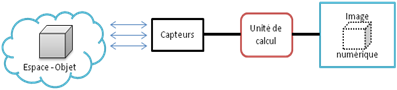
\includegraphics[width=0.5\textwidth]{model_scanner.png}
\caption{Schéma d'un scanner 3D}
\end{figure}
La numérisation tridimensionnelle a déjà fait ses preuves dans de nombreux domaines, notamment dans l’architecture (réalisation de plans de géomètre), la médecine (fabrication de prothèses personnelles) mais aussi les multimédia tels que les jeux vidéo et films.

\chapter{Etat de l'art}
Il existe 2 grandes catégories de scanner tridimensionnel :
\begin{itemize}
\item Les scanners de lieux/espaces permettant, par exemple, de numériser un local. 
\item Les scanners d’objets (catégorie étudiée dans ce projet ci-après).
\end{itemize}

\section{Les yeux, deux caméras.}
Comme pour beaucoup de technologies, la nature nous apporte une solution : les yeux. En effet, c’est grâce à nos deux yeux que nous pouvons visualiser le monde qui nous entoure en 3 dimensions. Cette technique s’appelle la stéréoscopie.\cite{stereo,raspberry}
\\
Cela fonctionne selon le principe de soustraction d’image. En effet, chaque œil joue le rôle d’une caméra. À un moment donné t, les yeux prennent chacun une photo. Grâce à un algorithme de traitement d’images, les images sont soustraites l’une de l’autre afin d’obtenir une image de ‘contours’ : tout objet se situant dans le lointain disparaîtra lors de la soustraction car l'angle au sommet du triangle caméra-1 – objet – caméra-2 étant très petit, les côtés de ce dernier seront quasiment parallèles et l'objet lointain sera donc représenté par le même pixel (x,y) sur les deux images. Tandis que nous observerons une sorte de contours pour les objets proche des caméras, car le triangle caméra-1 – objet – caméra-2 sera bien plus court et l'objet sera donc représenté par des pixels différents sur les images.
\begin{comment}
\begin{figure}[h!]
\begin{minipage}{.5\textwidth}
	\centering
	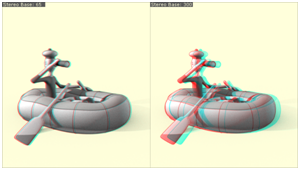
\includegraphics[width=0.5\textwidth]{image_stereo.png}
	\caption{\label{fig:image_stereo.png}Source 2.}
\end{minipage}%
\begin{minipage}{.5\textwidth}
	\centering
	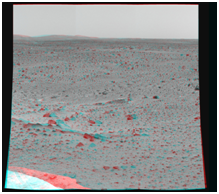
\includegraphics[width=0.5\textwidth]{image_stereo_mars.png}
	\caption{\label{fig:image_stereo_mars.png}Source 3.}
\end{minipage}
\end{figure}
\bibitem{3dgeeks} \url{http://3dgeeks.com/index.php?ct=articles&action=file&id=116}
\bibitem{nasa} \url{http://www.nasa.gov/images/content/54686main_full-analgyph.jpg}
\end{comment}
À l’aide d’un calibrage préalable et de la connaissance de la distance séparant les caméras et la distance séparant les pixels d’un même point de l'objet, il nous devient possible de calculer la distance séparant l’objet des caméras.
\\
\\
Cette technique est relativement complexe à élaborer : il faut intégrer les images obtenues par soustraction en faisant tourner l'objet, chaque image n'étant pas celle d'une simple intersection avec un plan ou d'une simple projection.

\section{Profil par contraste.}
Cette technique consiste à photographier l'objet illuminé par une source intense confondue avec l'objetif (en pratique, un flash annulaire autour de celui-ci) : l'objet apparaît totalement blanc par rapport au fond noir; il suffit de répéter l'opération en faisant tourner l'objet. Le procédé nécessite de l'espace suffisant derrière l'objet pour que le fond reste relativement sombre et ne détecte aucune concavité, ce qui est un gros handicap.

\section{Projection structurée lumineuse.}
Cette technique consiste à projeter des patterns lumineux à l’aide d’un projecteur sur l’objet à scanner (exemple : tomographie : un laser tournant dans un plan vertical autour de l'objet se déplaçant selon un axe perpendiculaire au plan). Les caméras photographient de part et d'autre l’objet illuminé (voir figure \ref{proj_structuree}). Comme le projecteur et les caméras se situent en des positions différentes, les patterns lumineux projetés paraissent déformés pour la caméra. C’est donc à partir de ces déformations qu’il est possible de déterminer la forme de l'objet.\cite{clemson,Murale}

\begin{figure}[h!]
\centering
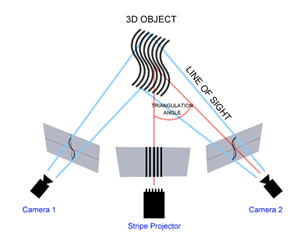
\includegraphics[width=0.5\textwidth]{proj_structuree.png}
\caption{Projecteur d'un rideau de lignes et deux caméras.\cite{clemson}}
\label{proj_structuree}
\end{figure}

Cette technique à l’avantage d’être rapide mais le désavantage d’être facilement perturbée par la lumière ambiante et nécessite un matériel coûteux.

\section{La télémétrie laser.}
Le télémètre laser mesure le temps que met une impulsion de lumière pour parcourir 2 fois la distance qui le sépare de l'objet. Sa précision est de l'ordre de 1 à 3 mm et est déterminée par celle de l'électronique embarquée qui doit mesurer le déphasage (retard) entre le train d'impulsions émis et celui reçu : 3,3 nanosecondes pour un objet à 50 cm de distance. Les mesures sont répétées en faisant osciller le télémètre autour d'un axe horizontal et tourner l'objet sur 360 degrés.

\section{Une caméra et deux lasers.}
Cette technique fonctionne grâce à 2 lasers, une caméra ainsi qu’une plateforme tournante. Les lentilles des lasers focalisent le rayon en un rideau vertical, ce qui laisse apparaître une ligne sur l’objet. La caméra prend une photo de l’objet lorsque les lasers sont allumés, ainsi que lorsqu’ils sont éteints. On procède ensuite à une soustraction des deux images précédemment obtenues afin de ne conserver que les traces lumineuses
produites par les lasers (voir figure \ref{laser_scanner}). Connaissant l’orientation des lasers, la distance qui les sépare ainsi que la distance au centre de la plateforme, il nous est possible de calculer la position exacte de chacun des points illuminés par les lasers. L’opération est répétée un certain nombre de fois, selon la qualité de l’image numérique souhaitée. L'utilisation de deux lasers permet notamment de corriger les effets de l'ambiance lumineuse, mais aussi d'obtenir deux tranches de l'objet par position, réduisant ainsi le nombre de rotations\footnote{C'est la rotation du plateau qui est la plus coûteuse en temps dans l'acquisition de points 3D.} à effectuer pour une résolution équivalente; et permet \cite{dsls} de distinguer les zones de l'objet qui pourraient être invisibles pour une seule caméra car cachées par des parties saillantes de l'objet : la caméra voit les lignes de contour formées par les deux lasers sous des angles différents; cette solution est moins coûteuse que disposer deux caméras de part et d'autre d'un laser (voir figure \ref{proj_structuree}).

\begin{figure}[h!]
\centering
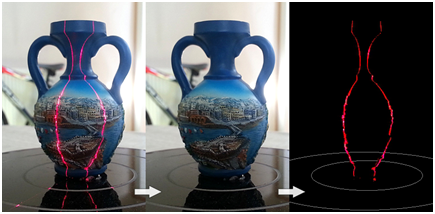
\includegraphics[width=0.9\textwidth]{laser_scanner.png}
\caption{Scanner à deux lasers\cite{rubicon}}
\label{laser_scanner}
\end{figure}
Cette technique n'est pas nouvelle : dans leur inventaire des méthodes utilisant des lasers, Forest et Salvi\cite{forest2002,forest2004} citent Sato (1982)\cite{sato} en exemple.\\
Nous exploitons cette technique dans notre projet.

\chapter{Méthodes implémentées}
\section{Le hardware}
Pour le prototype, nous allons devoir assembler les éléments suivants :
\begin{enumerate}
\item Deux diodes laser (faisceau plan);
\item Une caméra/appareil photo numérique/webcam;
\item Un moteur pas-à-pas ainsi qu'un contrôleur;
\item Un arduino utilisant un processeur ATmega de la firme Atmel\cite{ATmega}.
\end{enumerate}
\subsection{Diodes lasers}
Il sera fait usage de diodes lasers de faible puissance (classe 2 ou 3) afin d'en assurer en toutes circonstances l'inocu\"{i}té pour les yeux des opérateurs et des spectateurs. Elles sont pourvues d'une lentille projetant la lumière émise sous forme d'une ligne et non d'un point, ce qui permet l'usage de diodes de classe 3 (max. 5 mW).
Leur étude et leur mise en \oe uvre sont reprises en annexe \ref{diodes-laser}.

\subsection{Caméra}
La solution la plus simple est d'utiliser une webcam plutôt qu'un appareil photo; mais cela présente deux défauts : la résolution est limitée (maximum 2 Mpixels - les résolutions supérieures affichées par certains constructeurs sont obtenues par interpolation)\footnote{Exemple : webcam Microsoft Lifecam HD3000 : 1280x720 soit 0,92 MPixels} et un plan image (capteur) mal défini.
A titre de comparaison, le projet Rubicon (\cite{rubicon}) utilise un capteur Aptina MT9P006 de 5 Mpixels.
\\
L'utilisation d'une webcam pour prendre des photos est un contre-emploi; la webcam est conçue pour fournir environ 30 images par sec.; ses capacités de traitement limitent donc la définition des images, ce qui ne pose pas de problème pour un usage en tant que webcam, compte tenu d'autres contraintes telles que taille d'un écran (HD 1080p : 2 MPixels) et bande passante...
\\
Les appareils photo réflex numériques n'ont pas ces inconvénients, mais le protocole de communication USB auquel ils répondent est propriétaire et rarement divulgué : ces appareils ne respectent en particulier pas, comme les webcams récentes, les spécifications USB video device class (UVC) ({\cite{UVC}}). Mais tous les appareils photo numériques et de nombreux GSM supportent le protocole PTP (Picture Transfer Protocol) : avec la librairie libgphoto2 il devient possible de commander de nombreux appareils à partir d'un PC (\cite{gPhoto,libgp2,cremote})\footnote{Testé : Canon Powershot SX100IS 8 MPixels}. L'inconvénient de cette solution est sa lenteur : elle ne sera pas retenue.
\subsection{Moteurs pas-à-pas}
Deux types de moteurs pas-à-pas ont retenu notre attention(\cite{stepper}) : les unipolaires et les bipolaires. Tous ont un stator pourvu d'un nombre pair d'enroulements, nombre qui va déterminer le nombre de pas. Le schéma simplifié de la partie gauche de la figure \ref{unipolar} représente deux enroulements : les moteurs unipolaires se distinguent par la présence d'une connection (1 et 2) au milieu de ceux-ci; ces deux connections sont parfois reliées entre elles (5 fils) ou non (6 fils). L'alimentation des moteurs unipolaires est plus simple: seule la moitié de chaque enroulement est excitée à la fois; le passage d'un pas au suivant ne nécessite pas l'inversion du courant, mais simplement l'excitation d'un autre demi-enroulement; son couple est évidemment deux fois moindre que celui du moteur bipolaire équivalent. Un moteur monoplaire à 6 fils peut être utilisé comme bipolaire en ne connectant pas les fils 1 et 2.
\begin{figure}[h!]
\centering
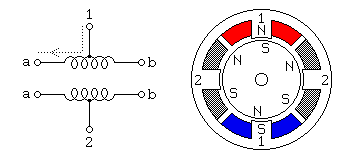
\includegraphics[width=0.4\textwidth]{2anim.png}
\caption{Schéma d'un moteur unipolaire (\cite{jones_stepper})}
\label{unipolar}
\end{figure}
\begin{itemize}
\item \textbf{Moteurs 200 pas 12 V, à 5 ou 6 fils} (Figure \ref{Tandon}) \\
Il s'agit de moteurs qui équipaient les lecteurs de floppy disks 5$\sfrac{1}{4}''$ (fabricants Tandon et Japan servo co). Très endurants, ils consomment beaucoup (150 à 800 mA) pour assurer un couple de maintien élevé. Leur définition est limitée (1,8° par pas).
\item \textbf{Moteur 64 pas 5 ou 12 V, à 5 fils} (Figure \ref{28BYJ-48}) \\
Peu coûteux car fabriqués en grandes quantités, ces petits moteurs consomment peu et obtiennent néanmoins un couple et une définition (0,088° par pas) élevés grâce à la présence d'un engrenage réducteur $\sfrac{1}{64}$. Il faut donc 4096 pas pour accomplir un tour.
\end{itemize}
\begin{figure}[h!]
\begin{minipage}{.5\textwidth}
	\centering
	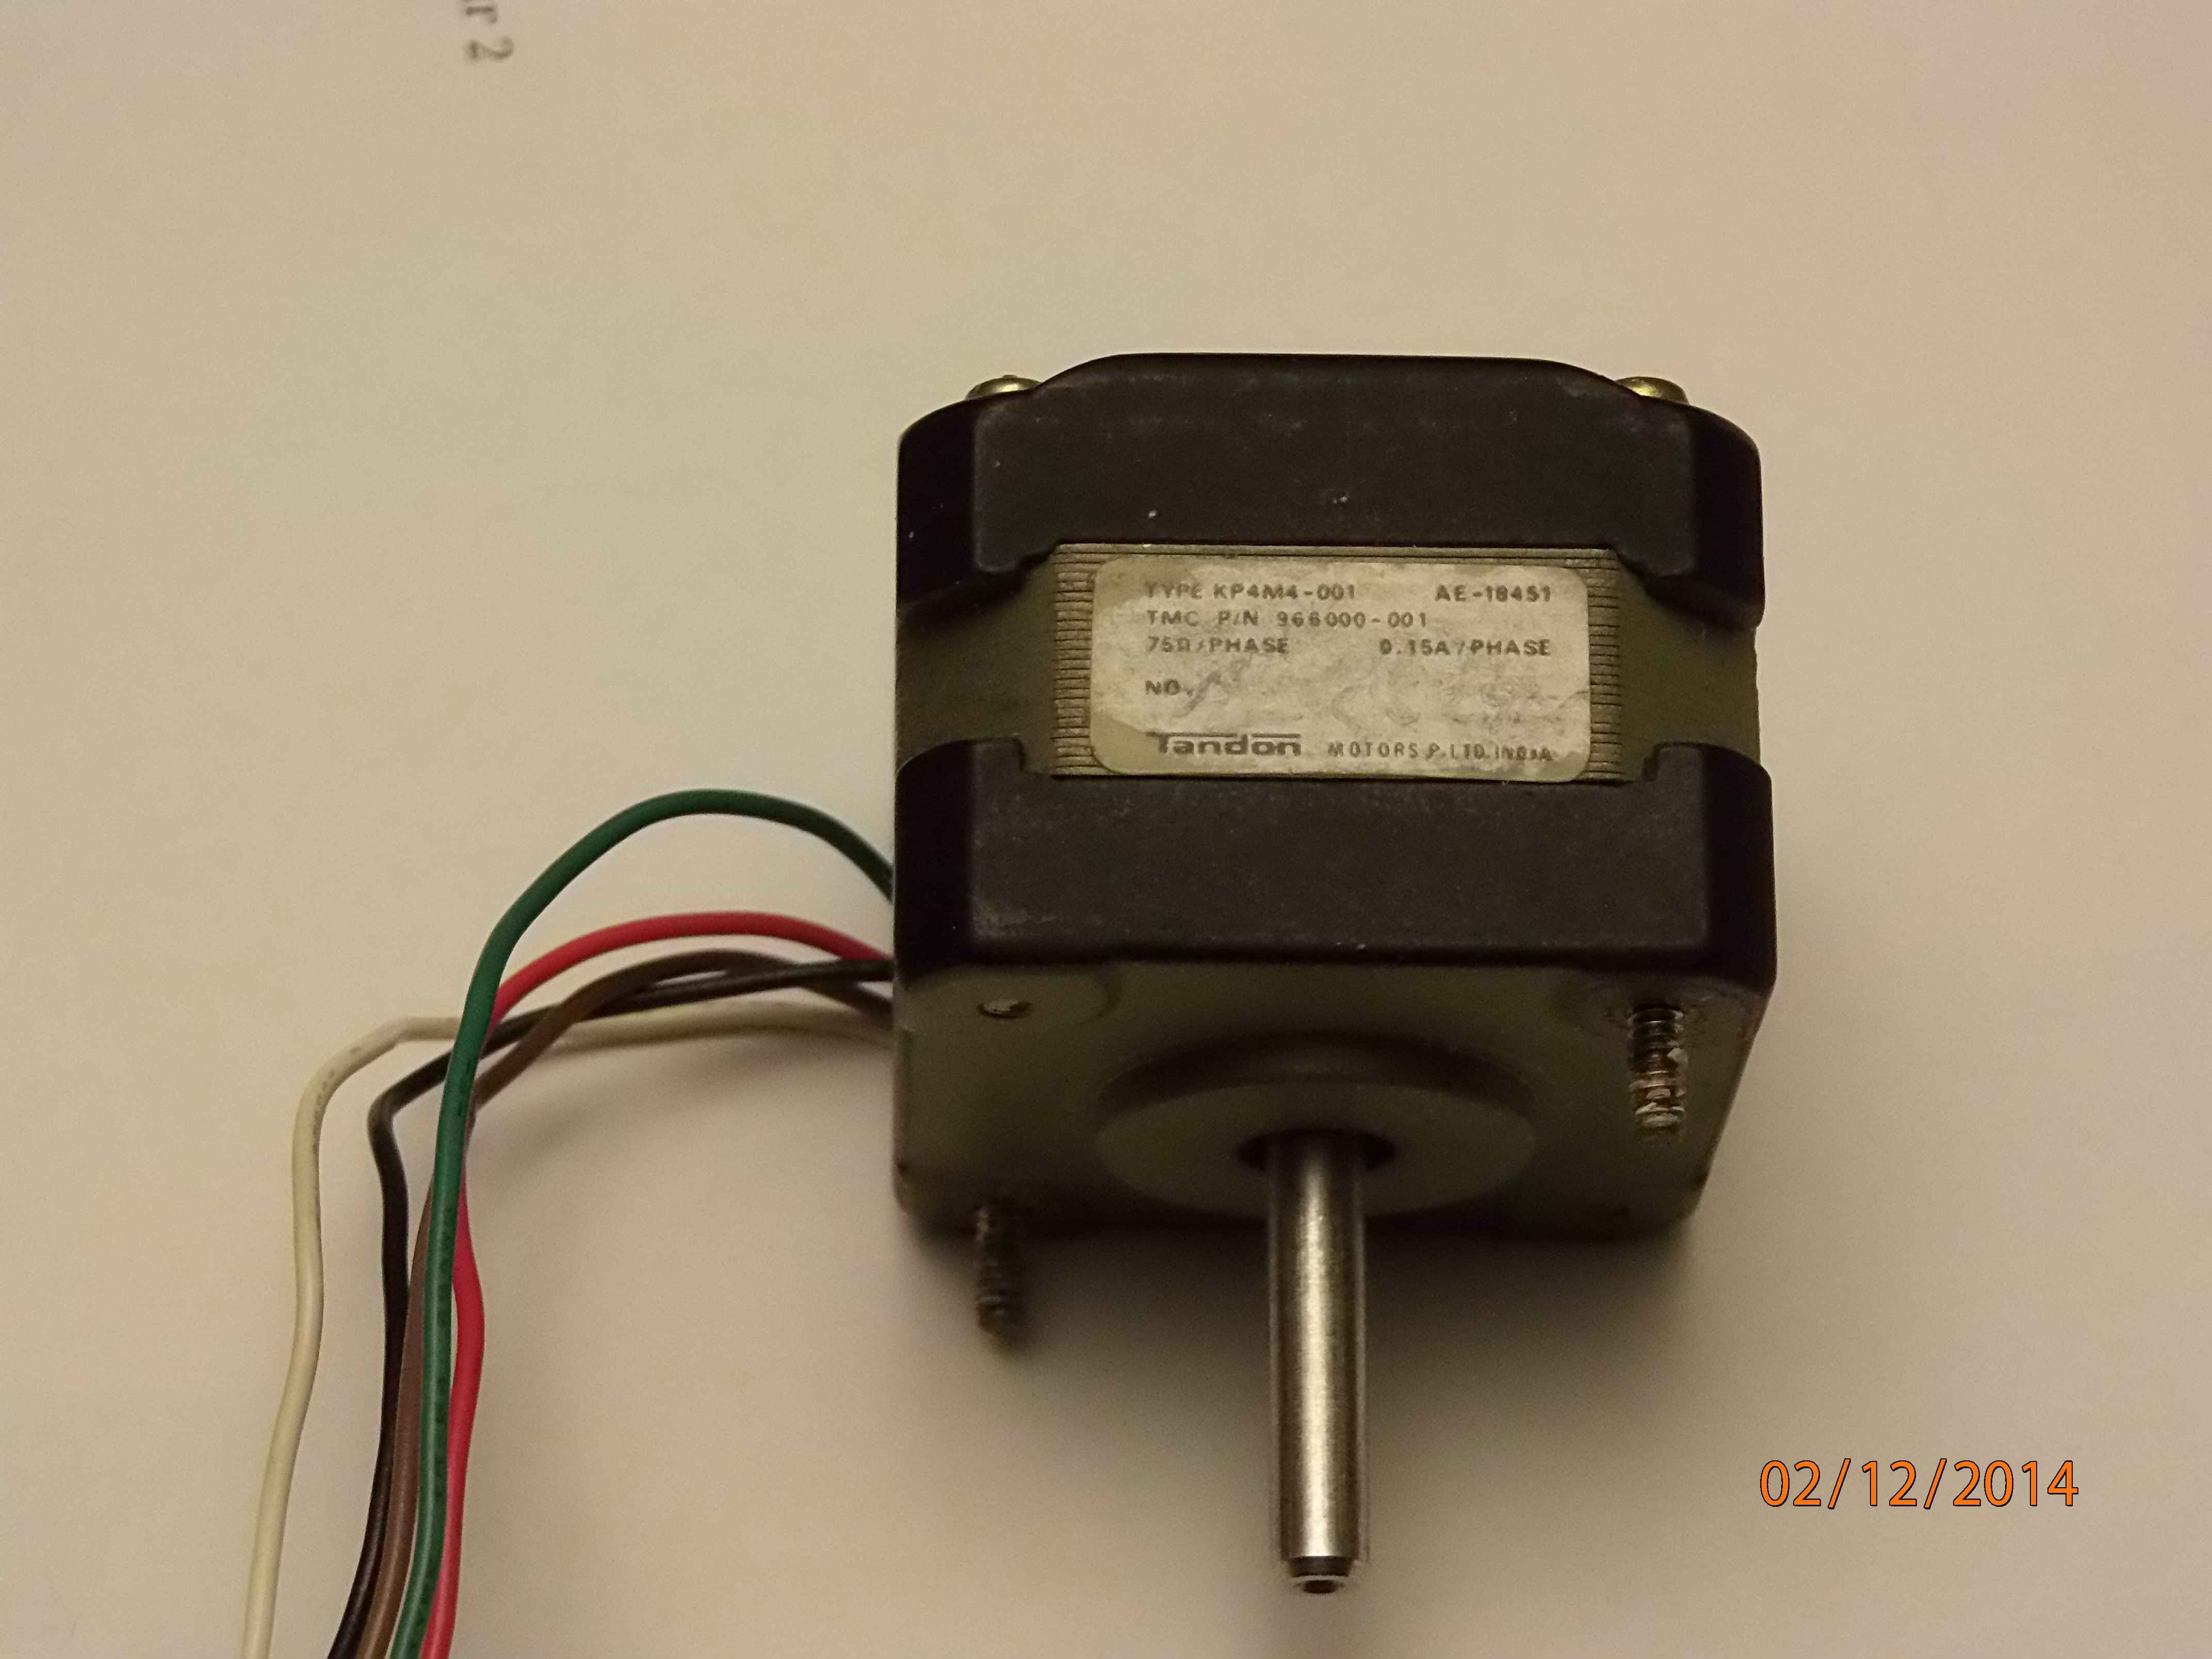
\includegraphics[width=0.7\textwidth]{Tandon.JPG}
	\caption{Moteur 200 pas, 12 V}
    \label{Tandon}
\end{minipage}%
\begin{minipage}{.5\textwidth}
	\centering
	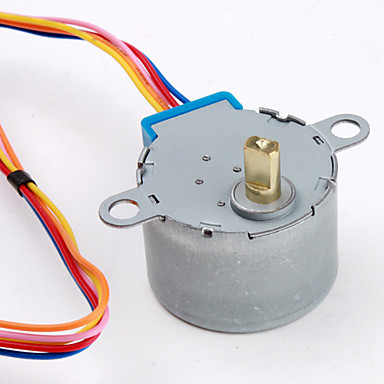
\includegraphics[width=0.5\textwidth]{stepper5V.jpg}
	\caption{Moteur 64 x 64 pas, 5 V - 28BYJ-48}
    \label{28BYJ-48}
\end{minipage}
\end{figure}
\subsection{Les contrôleurs des moteurs pas-à-pas}
Les contrôleurs des moteurs unipolaires sont très simples : il suffit d'un circuit rassemblant plusieurs transistors darlingtons (un ULN2003 par exemple).\\
Sans entrer ici dans les détails, signalons que les contrôleurs de bipolaires sont plus complexes(\cite{stepctrl}). Nous utilisons le circuit Easydriver réalisé autour du chip A3967 d'Allegro Microsystems.
\subsection{Construction}
\begin{comment}
Un premier prototype a été réalisé avec un moteur 28BYJ-48 sur un assemblage d'élements métaliques de récupération formant une plateforme très stable. Les 4096 pas avec 4096 allumages et extinctions des diodes et 2x4096 enregistrements d'images par la webcam du PC\footnote{i7-3632QM 2,2 GHz sous Linux Mint 17 64 bits} (mais sans traitement de celles-ci) sont effectués en 11 minutes.\\

\begin{figure}[h!]
\centering
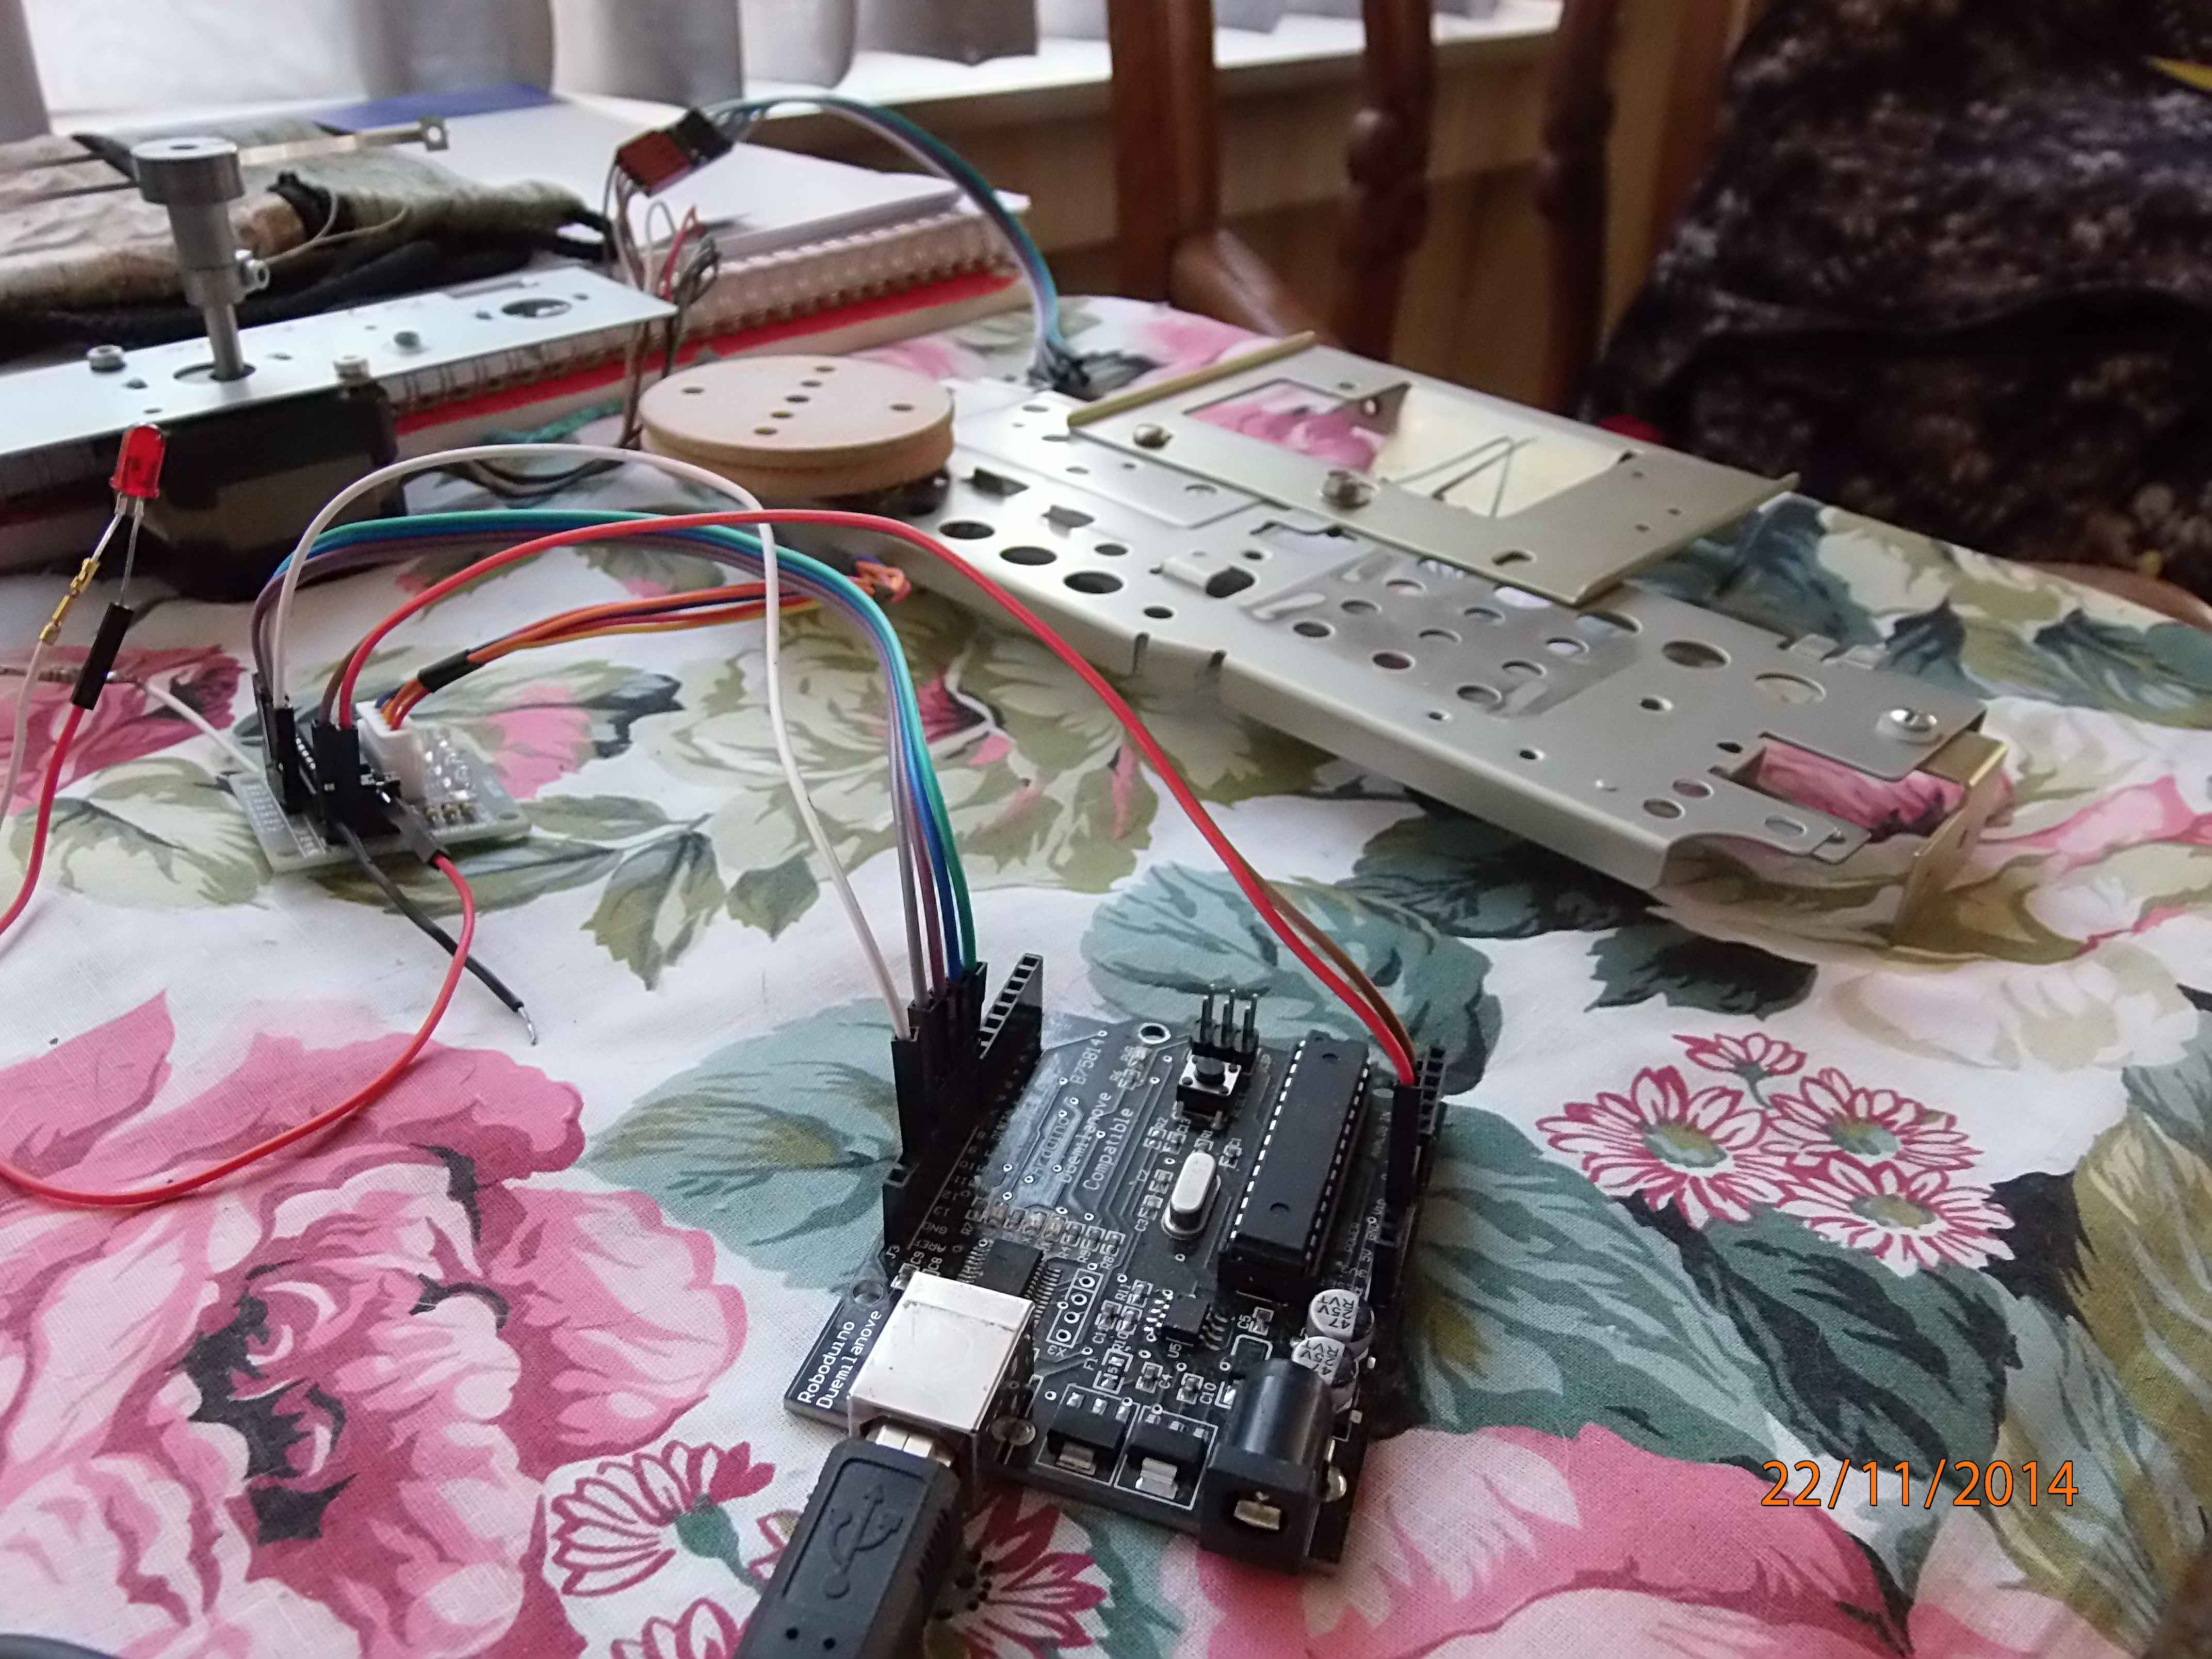
\includegraphics[width=0.4\textwidth]{proto1.JPG}
\caption{Premier prototype}
\label{proto1}
\end{figure}
\end{comment}
Le prototype utilise une webcam Logitech Carl Zeiss Tessar HD 1080p (figure \ref{proto}). À chaque pas, la webcam capture 3 photos: une avec le laser gauche allumé, la seconde avec les deux lasers éteints et la dernière avec le laser droit allumé. Une reconstruction de l'objet dans son entièreté est ensuite élaborée. La création de ce prototype nous permet d'appliquer certaines techniques de calibrage (principalement physiques) et de nous pencher plus concrètement sur les problèmes de calculs de distances. Un algorithme de triangulation a été développé et testé sur ce tirage.

\begin{figure}[h!]
\centering
\includegraphics[width=0.8\textwidth]{proto2.JPG}
\caption{Second prototype}
\label{proto}
\end{figure}

\section{Le software sur l'arduino}
Le rôle de l'arduino est réduit à la commande du moteur pas-à-pas via son contrôleur et l'allumage des lasers. Son programme se limite donc à la réalisation d'un interprêteur de commandes reçues du PC par une liaison série. Son code, qui n'est évidemment pas présent sur la machine virtuelle tournant sur le PC, est repris en annexe \ref{code-arduino}.

\section{Le software sur le PC}
Les fonctions principales du logiciel Python sur le PC sont :
\begin{enumerate}
\item Calibrage du système afin d'établir la relation entre les coordonnées d'un point dans le plan de l'image 2D et les coordonnées 3D du point correspondant sur l'objet;
\item Acquisition d'images de l'objet à scanner à chaque étape de rotation de la plateforme;
\item Traitement des images pour en extraire les tracés laser (à l'aide de la libraire OpenCV \cite{openCV});
\item Calcul des coordonnées tridimensionnelles des points de l'image précédement obtenue par triangulation afin de construire un nuage de points (et simplification éventuelle du nombre de points);
\item Relier ces points en un réseau (meshing); plusieurs méthodes ont été mises en \oe uvre pour pouvoir les comparer;
\item Compléter et éventuellement corriger ce réseau en l'égalisant (smoothing) pour reconstituer la surface (la représentation et les manipulations de ce nuage de points se fera à l'aide de la librairie opengl \cite{opengl}).
\end{enumerate}
Ce processus sera itératif afin d'ajuster les paramètres en vue d'améliorer le résultat.

\subsection{Calibrage}
Le calibrage peut être constructif ou software ou une combinaison des deux.
\subsubsection{Calibrage constructif}
Il faut positionner de façon précise les lasers qui émettent un "rayon plan", la caméra et le plateau portant l'objet à scanner et mis en rotation par le moteur pas-à-pas.
\begin{enumerate}
\item Régler les lasers de telle sorte que l'intersection de leurs plans de projection coïncide avec l'axe de rotation du plateau.\\
Pour faciliter ce réglage, on commence par s'assurer (avec un niveau d'eau) que le plateau est parfaitement horizontal; on matérialise ensuite l'axe de rotation à l'aide d'un fil à plomb; il suffit alors de régler les diodes pour que leurs "rayons laser" illuminent le fil à plomb sur toute sa hauteur, en commençant par vérifier que leur intersection sur le plateau coïncide avec le centre de rotation de celui-ci. Il faut ensuite mesurer les angles d'orientation des lasers.
\item Positionner la caméra de telle façon que le centre du capteur soit sur la bissectrice de l'angle formé par les deux diodes laser et le centre de rotation comme sommet, et que le capteur soit perpendiculaire à cette bissectrice.
\item Il ne reste plus qu'à mesurer la position de la caméra, du centre du plateau et des lasers (par rapport au pied de la camera sur le sol), ainsi que les angles d'orientation des lasers et de la camera.
\end{enumerate}
\subsubsection{Calibrage software}
Pour palier la grande difficulté de réaliser correctement tous les réglages et mesures du calibrage constructif, un calibrage software est nécessaire. Celui-ci consiste à:
\begin{enumerate}
\item Positionner les lasers de telle façon qu'ils passent par le centre du plateau et mesurer la position tridimensionnelle du centre du plateau, de la caméra et des lasers.
\item Capturer un triplet d'images du plateau vide: celle de gauche où figure la ligne tracée par le laser de gauche, l'image dit "de fond" où aucun laser n'est allumé, et enfin celle de droite où figure la ligne tracée par le laser de droite. Il suffit alors d'extraire les tracés laser et de déterminer leur intersection qui correspond au centre du plateau dans le monde 2D. Grâce à ces tracés lasers sur le plateau, on devient capable de déterminer le centre du plateau sur les images (leur intersection), ce qui nous permet alors de faire une correspondance avec la position 3D du centre de la table déterminée à l'étape précédente. (voir Figure \ref{fig:softcalib})
\item Connaissant la position réelle du centre du plateau, nous pouvons réaliser une correspondance entre le point 2D déterminé précédement et le point 3D mesuré lors de la première étape. Nous devenons alors capable de déterminer l'orientation de la camera par rapport aux plans horizontal et vertical. En effet, nous possédons une correspondance entre le monde 2D et 3D pour le centre du plateau et nous connaissons la position réelle de la caméra; nous pouvons donc tracer le vecteur bisecteur partant du capteur de la camera en joignant le centre du plateau (comme si la camera était centrée sur le centre du plateau). Il suffit ensuite de pivoter ce vecteur de façon à ce qu'il corrige l'offset vertical et horizontal du centre du plateau 2D par rapport au centre de l'image. Nous obtenons alors l'orientation réelle de la camera.

\begin{figure}[h!]
  \centering
  \begin{subfigure}[b]{0.59\textwidth}
    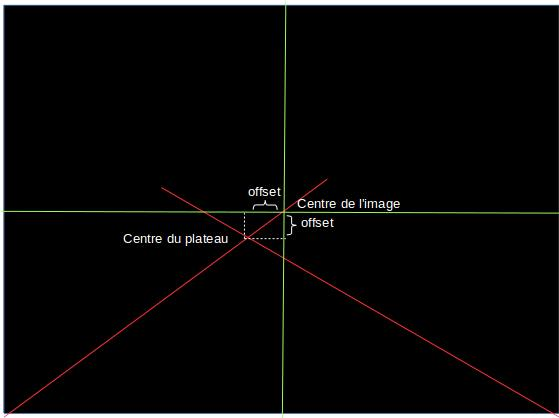
\includegraphics[width=\textwidth]{calibration_jpg.jpg}
    \caption{Calibration du centre du plateau}
  \end{subfigure}
  \begin{subfigure}[b]{0.39\textwidth}
  	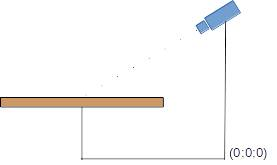
\includegraphics[width=0.9\textwidth]{plateau_jpg.jpg}
  	\caption{Schéma}
  \end{subfigure}
  \caption{\label{fig:softcalib} Calibration software du système}
\end{figure}

\item Il ne reste plus qu'à déterminer l'orientation des lasers. Pour cela, nous faisons l'hypothèse que les lasers sont alignés avec la caméra. Connaissant la position du centre du plateau, de la caméra, des lasers et l'orientation de la caméra, il devient aisé de modéliser les plans verticaux que tracent les lasers. En effet, nous connaissons le vecteur vertical ainsi que le vecteur horizontal partant de la position du laser et joignant le centre du plateau. Nous sommes donc capables de déterminer les angles que font ces plans avec le plan vertical du repère. Il s'agit des angles respectifs des lasers.
\end{enumerate}

\subsection{Acquisition et extraction des tracés laser}
La caméra prend une photo de l’objet pour chaque laser allumé individuellement, ainsi qu'une photo lorsqu’ils sont éteints. La soustraction d'une image laser allumé et lasers éteints permet d'extraire grossièrement le tracé laser en question. Il faut donc ensuite appliquer tout une série de filtres afin d'épurer ce tracé. Pour ce faire, nous appliquons des filtres de couleurs RGB, de saturations HSV ainsi que des filtres basiques de seuil, de flou Gaussien et médian. Finalement, nous réduisons le tracé à un unique pixel en largeur grâce à une moyenne pondérée en fonction de l'intensité du pixel par rapport à sa position.

\subsection{Triangulation}
C'est sous ce nom que certains auteurs (\cite{Forsyth} par exemple) nomment la recherche des coordonnées spatiales.\\
Cette opération a pour but de transformer chaque point 2D du tracé laser extrait précédement en points 3D. Cela consiste donc a déterminer l'intersection du plan laser (déterminé par ses deux vecteurs directeurs) et du rayon lumineux provenant du "plan image" et percutant le capteur de la camera. Il s'agit donc de résoudre un simple système de 3 équations à 3 inconnues:\\

\begin{equation}
\begin{pmatrix}
x\\ y\\ z
\end{pmatrix}
=
\begin{pmatrix}
-pixel_x & \alpha_x & \beta_x \\
-pixel_y & \alpha_y & \beta_y \\
-camDist & \alpha_z & \beta_z
\end{pmatrix}^{-1}
*\textbf{R}*
\begin{pmatrix}
\gamma_x \\
\gamma_y \\
\gamma_z
\end{pmatrix}
\end{equation}
où $\alpha$ et $\beta$ sont les deux vecteurs directeurs du plan laser, \textbf{R} est la matrice d'orientation de la camera et $\gamma$ est la différence entre la position de la caméra et la position du laser en question.
Une fois les points 3D obtenus, il ne reste plus qu'à les faire tourner du nombre de pas déjà effectués par le plateau autour du centre de celui-çi.
On obtient alors un nuage de points 3D.

\begin{figure}[H]
\centering
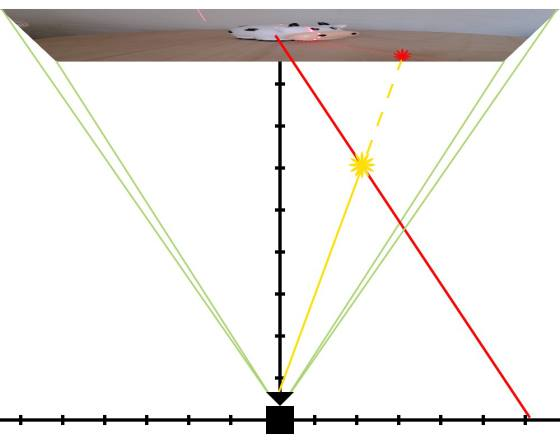
\includegraphics[width=0.5\textwidth]{triangulation_jpg.jpg}
\caption{Triangulation}
\label{unipolar}
\end{figure}

\subsection{Ramer-Douglas-Peucker}
Il est ensuite possible d'appliquer un filtre à la fin de la triangulation, pour réduire le nombre de points. La réduction de la densité du nuage de points permet de considérablement diminuer le temps de maillage, mais risque en contrepartie de provoquer plus de trous dans la surface reconstruite\footnote{Ce résultat sera discuté plus loin}. En outre, on souhaite supprimer des points non pas pour en atteindre un nombre fixe, mais pour garder les points les plus significatifs. L'algorithme de simplification de ligne de Douglas-Peucker\cite{douglaspeucker} a été créé dans ce but. Nous l'avons implémenté, en sortie de l'étape de triangulation.

L'algorithme est appliqué sur chaque tranche correspondant aux points illuminés par un laser sur une photo. Nous savons donc que tous ces points sont dans le même plan. On les trie verticalement et on applique l'algorithme de Douglas - Peucker:

\begin{enumerate}
	\item On trouve le point $M$ le plus éloigné de la droite $D$ passant par les deux points extrêmes $P_1 et P_2$ de la polyligne
  \item Si la distance de $M$ à $D$ est inférieure à un certain seuil (paramètre de la procédure), on supprime tous les points intérieurs et l'algorithme s'arrête (\textit{plus aucun point n'est significatif})
  \item Sinon, on répète l'algorithme récursivement sur les deux polylignes formées par les points entre $P_1$ et $M$ et entre $M$ et $P_2$ (\textit{$M$ est significatif})
\end{enumerate}

\subsection{Représentation en 3D}
A ce stade, nous disposons d'un nuage de points en 3D. Cependant, les applications 3D utilisent usuellement des volumes, notamment pour déterminer ou passerait la lumière, par où de l'eau s'écoulerait, ... Plusieurs étapes sont nécessaires pour transformer cet ensemble de points en un solide.(\cite{shapiro}-chap.13)\\
Deux représentations sont possibles : un réseau de mailles (meshes) reliant ces points ou un ensemble de petits cubes (voxels), à la manière d'une image bitmap. Il est possible de passer d'une représentation à l'autre par rastérisation.\\
Pour constituer ces représentations, une étape importante sera d'éliminer tant que faire se peut les points "parasites" ("bruit").
\subsubsection{Voxelisation}
Un voxel est un pixel en 3D : sa valeur binaire indique si le cube dans l'espace qu'il représente appartient ou non à l'objet.(\cite{Voxelization,basdogan,pulli})\\
La technique de base utilisée pour éliminer les points parasites consiste à découper l'espace ("space carving") en domaines (de grands voxels en fait). Pour rafiner cette partition, les voxels présents sur les contours des domaines sont décomposés en 8 voxels plus petits de façon itérative; le programme les gère dans un octree (arbre dont chaque noeud a 8 enfants). Lorsqu'on a atteint la définition maximale souhaitée (la taille minimale des voxels) sur tous les contours, on a obtenu un modèle "voxelisé" de l'objet.
\subsubsection{Maillage}
L'étape de maillage (meshing en anglais) consiste à relier les points en un réseau de polygones (idéalement des triangles) qui formeront un polyèdre. 
Il s'agit donc de trouver les points de la surface de l'objet qui sont effectivement reliés, et d'ignorer les espaces vides.\\
Une multitude d'algorithmes ont été proposés pour reconstituer ce maillage.
Plusieurs classifications de ses algorithmes ont été proposées, notammment dans \cite{Mencl} et \cite{IPD}. L'inventaire le plus récent à notre connaissance date de 2014\cite{Berger}.\\
Nous avons retenu quelques algorithmes et les avons comparés; ils correspondent à des approches différentes :
\begin{itemize}
\item \textbf{Les approches sculptant la surface}; après avoir décomposé l'espace en cellules, elles opèrent une sélection de celles-ci, soit par rapport à la surface, soit par rapport au volume du solide :
\begin{itemize}
\item Sélection "orientée surface" : elles recherchent les cellules traversées par la surface du solide et suppriment celles, trop grandes, qui sont dans le solide ou en dehors; l'algorithme "alpha-shape" (voir § \ref{alpha-shape}) appartient à cette cathégorie.
\item Sélection "orientée volume" : elles supriment les cellules qui n'appartiennent pas au volume; l'algorithme "ball pivoting" (voir § \ref{BPA}) appartient à cette catégorie.
\end{itemize}
\item \textbf{Les approches faisant grossir des régions}; les algorithmes "Delaunay-based Region-growing" (\cite{DBRG}) et "Intrinsic Property Driven" (\cite{IPD} et § \ref{Intrinsic}) font partie de cette catégorie.
\end{itemize}
\paragraph{Delaunay et alpha-shape}\label{alpha-shape}
La reconstruction d'une surface à l'aide de facettes triangulaires se nomme, sans originalité, "triangulation". S'il en existe plusieurs à partir d'un même nuage de points, une seule d'entre 
elle est appelée \textbf{triangulation de Delaunay} (\cite{Delaunay}, \cite{2algo} et \cite{edelsbrunner}). Un triangle de Delaunay est tel qu'il n'y a aucun point à l'intérieur de son cercle circonscrit.\\
Une fois les triangles construits, il faut éliminer ceux qui ne font pas partie de la surface, soit parce qu'ils sont à l'intérieur du solide, soit parce que, reliant des points d'une partie concave de la surface, ils sont à l'extérieur du solide (figures \ref{Delaunay-avant} et \ref{Delaunay-apres}).\\
Un des algorithmes utilisés se base sur la valeur d'un \textbf{paramètre de distance euclidienne \(\alpha\)} (laquelle a été fixée selon des caractéristiques propres au nuage de points) :
si le rayon du cercle circonscrit du triangle est supérieur à \(\alpha\), il n'est pas pris en compte \cite{alpha}.\\
Une allégorie pour mieux comprendre ce paramètre est celle du bloc de crème glacée aux pépites de chocolat (\cite{glace}) : armés d'une cuillère,
nous creusons et retirons petit-à-petit la glace, en évitant les pépites; l'ensemble des pépites représente notre nuage de points et le rayon de notre cuillère correspond à \(\alpha\).
Plus le rayon est petit, plus de glace nous pourrons retirer sans toucher à des pépites pourtant très proches. Au contraire, si le rayon est trop grand, le bloc de glace restera intacte.
Ainsi, le paramètre \(\alpha\) détermine la distance à laquelle les points doivent se trouver les uns par rapport aux autres pour être reliés par l'algorithme (figures \ref{Delaunay-avant} et \ref{Delaunay-apres}).

Nous avons intégré l'algorithme de triangulation de la bibliothèque Vizualisation ToolKit (vtk \cite{vtk}), accessible dans l'interface graphique depuis le bouton \textit{Mesh with Delaunay3D}
\begin{figure}[h!]
\begin{minipage}{.5\textwidth}
	\centering
	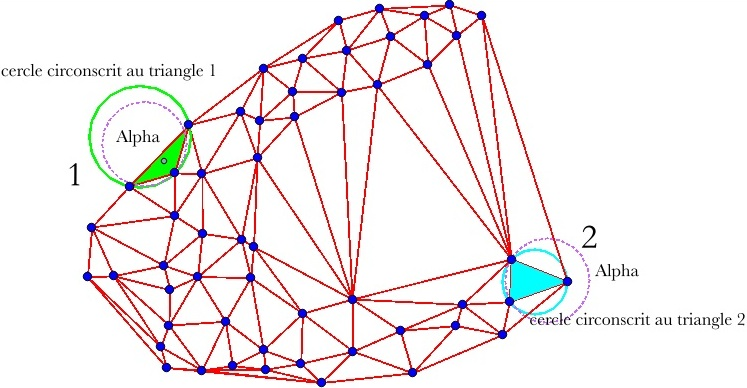
\includegraphics[width=1.1\textwidth]{Delaunay-avant.jpg}
	\caption{Avant suppression des triangles(\cite{glace})}
    \label{Delaunay-avant}
\end{minipage}%
\begin{minipage}{.5\textwidth}
	\centering
	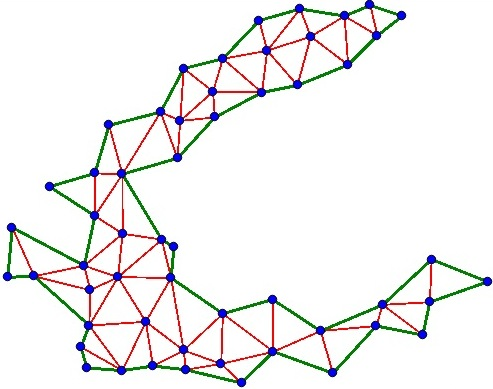
\includegraphics[width=0.7\textwidth]{Delaunay-apres.jpg}
	\caption{Complexe alpha résultant(\cite{glace})}
    \label{Delaunay-apres}
\end{minipage}
\end{figure}
\paragraph{Ball Pivoting}\label{BPA}
Un algorithme a retenu notre attention pour sa rapidité et la qualité de ses résultats sur nos jeux de données: le \textbf{Ball Pivoting Algorithm} (\cite{bpa} et \cite{Digne}). L'idée sous-jacente est simple: on choisit d'abord 3 points qu'on relie par un triangle. On fait ensuite pivoter virtuellement une boule d'un rayon $ \rho $ donné autour de chaque arête. Si la boule intercepte des points, on crée un nouvau triangle ayant pour sommets les deux sommets délimitant l'arrête autour de laquelle on tourne et le point dernièrement touché. L'algorithme se répète tant qu'il y a des points accessibles à partir des triangles déjà obtenus. S'il reste des points isolés, on en choisit 3 pour recommencer l'algorithme, jusqu'à ce qu'aucun point ne puisse être joint. L'algorithme est illustré en 2 dimensions à la figure \ref{fig:bpa-principle}. \'A condition de choisir des types des données efficaces pour la recherche spatiale, l'algorithme peut s'exécuter en un temps presque linéaire, et permet d'être utilisé sur des portions seulement du volume à reconstituer\cite{bpa}. Nous avons intégré l'implémentation libre en C++ de Julie Digne\cite{Digne}, chercheuse au FNRS, dans notre programme (accesible depuis le bouton \textit{Mesh with BPA}).

\begin{figure}[h]
	\centering
    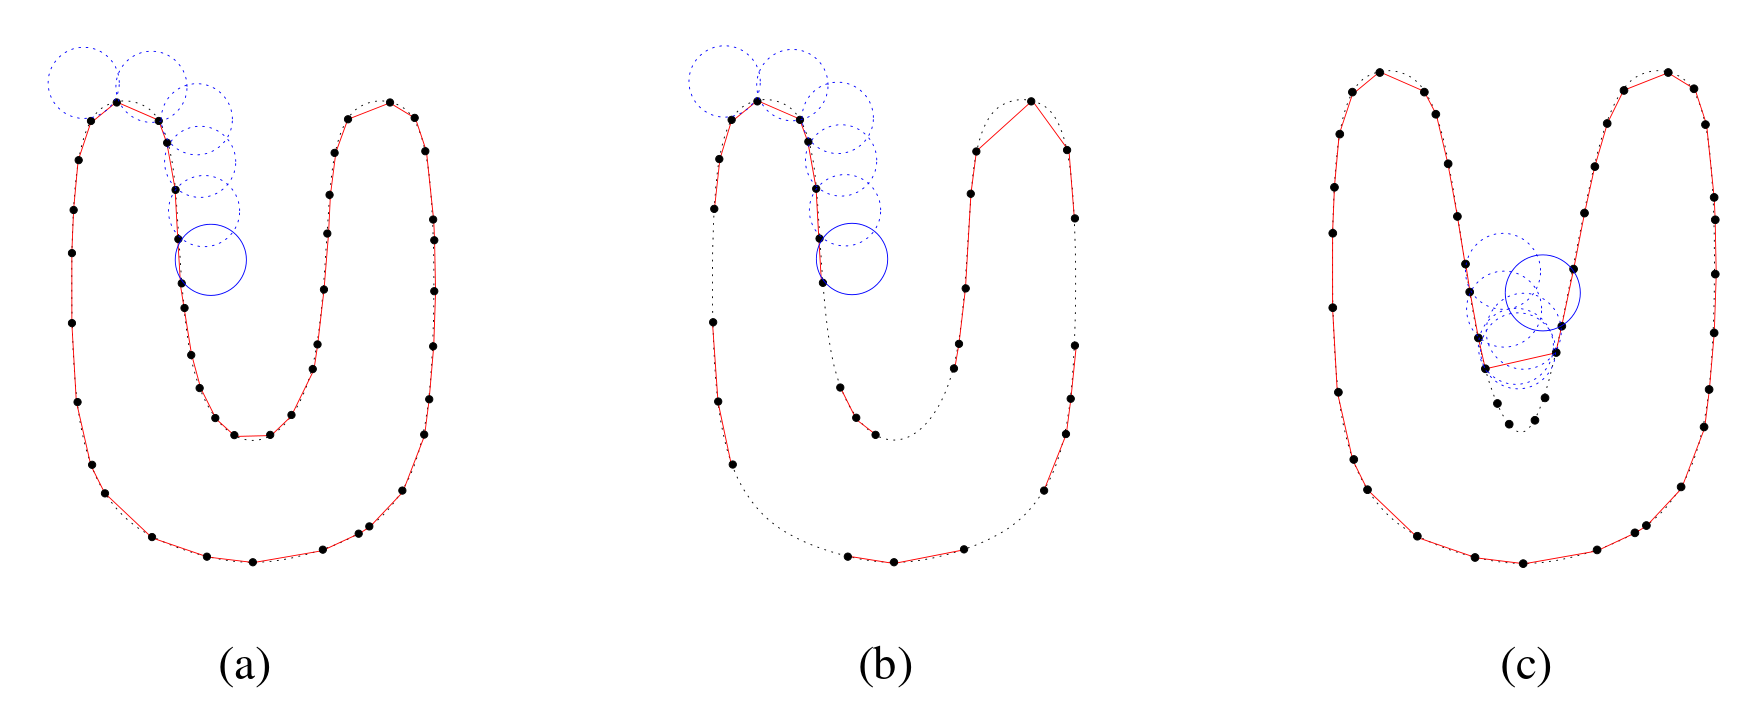
\includegraphics[width=\textwidth]{bpa-principle.png}
    \caption{\label{fig:bpa-principle} Principe du BPA illustré en 2D. a) Cas général. b) Les points sont trop espacés par rapport au rayon de la balle par endroit: formation de trous. c) Une concavité trop serrée empêche la balle de l'épouser parfaitement, des points sont ignorés. \textit{source: \cite{bpa}}}
\end{figure}

\paragraph{Intrinsic Property Driven}\label{Intrinsic}
Nous avons ensuite exploré l'algorithme guidé par les propriétés intrinsèques des triangles\cite{IPD}. L'algorithme commence comme le BPA, en choisissant un triangle de départ. Dans notre implémentation en Python, nous prenons le point le plus haut, et ses deux plus proches voisins. Chacune des arrêtes de ce triangle est placée dans la file des arrêtes actives. Tant qu'il y a des arrêtes dans cette file, on prend la première et on examine la taille des arrêtes adjacentes. On détermine ensuite le centre du triangle auquel elle appartient (\textit{Invariant: une arrête appartient au plus à deux triangles}), et on construit une région d'influence dans laquelle il est fortement probable de trouver un point pour former un nouveau triangle. Cette région est un triangle extrudé, formé par le centre du triangle auquel appartient l'arrête, et par deux points alignés chacun sur une droite passant par le centre du triangle de l'arrête et le point déterminant l'arrête. La distance de ces points au triangle original est proportionnelle à la taille des arrêtes avoisinnantes, d'où le nom de "propriétés intrinsèques". On prend le plus proche point dans cette zone d'influence, on forme deux nouvelles arrêtes formée par ce point et les deux points de l'arrête active, et on enfile les deux arrêtes ainsi obtenues. L'algorithme s'arrête donc quand on ne trouve plus de points dans la zone d'influence.

Pour la recherche de points dans l'espace, nous utilisons une structure de données nommée \texttt{VoxelSpace}. Il s'agit d'un ensemble de cubes de l'espace, de taille prédéfinie. On peut dès lors associer à chaque point $(x, y, z)$ de l'espace, un cube $(i, j, k)$. Cette technique permet de grandement réduire le nombre de points à examiner lors de la recherche du point le plus proche d'une position donnée, en ne parcourant que la liste des points des cubes adjacents. 

\begin{figure}[h]
	\centering
    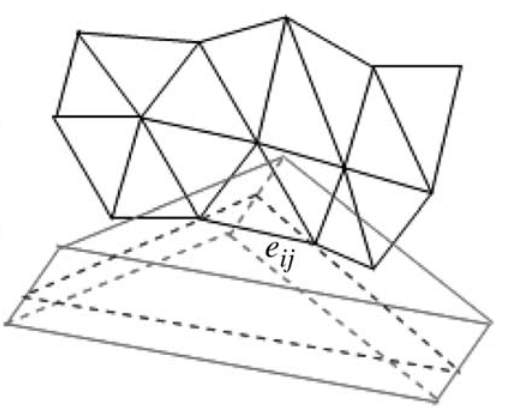
\includegraphics[width=.5\textwidth]{ipd-region.png}
    \caption{\label{fig:ipd-region} Région d'influence d'une arrête dans l'Intrinsic Property Drivern algorithm \textit{source: \cite{IPD}}}
\end{figure}

\subparagraph{Filtrage des triangles dégénérés}
L'algorithme précédent, bien qu'il nous permette de mailler tous les objets scannés, crée parfois des triangles dégénérés (ayant des côtés beaucoup plus longs que les autres), qui sont souvent provoqués par le bruit capté en amont dans la chaîne d'acquisition du programme. On peut cependant les enlever avec un intervalle de confiance statistique: on élimine tous les triangles dont au moins une arrête est en dehors des 99.9\% d'une distribution normale estimée à partir de la moyenne et de l'écart type de la longueur de toutes les arrêtes trouvées. On remarque qu'aucun triangle "important" (au sens où il influe sur notre perception de l'objet) n'est enlevé.


\subsection{Les outputs}
Le résultat du maillage est fourni dans un fichier au format .OBJ directement lisible par la plupart des logiciels de conception assistée par ordinateur.\\
En outre, le nuage de points peut aussi être sauvegardé sous le même format et relu ultérieurement pour recalculer un maillage.\\
Il en est de même des photos prises par la caméra, qui peuvent être gardées et rechargées pour être à nouveau traitées ultérieurement.

Remarquons en particulier le logiciel libre Meshlab\cite{meshlab}, qui permet de visualiser les volumes obtenus, et de leur appliquer des filtres ou des algorithmes de reconstruction. Nous pouvons ainsi observer les résultats des différents algorithmes avant de se lancer dans une étude plus détaillée.

\subsection{Interface du programme}

L'interface est sommaire mais contient tout le nécessaire. Les vues sont découpées en deux onglets. 

Le premier permet de lancer un scan (ce qui va lancer une calibration au préalable), et de voir le nuage de points se construire en temps réel. On peut en outre y exporter les nuages de points scannés, et lancer la reconstruction de surface par différents algorithmes.

Le second onglet permet d'entrer des paramètres de distances du matériel (distance de la caméra au plateau par exemple), ainsi que les chemins de fichiers pour l'enregistrement des photos de sauvegarde, la caméra ou l'arduino.

\begin{figure}[h]
	\centering
    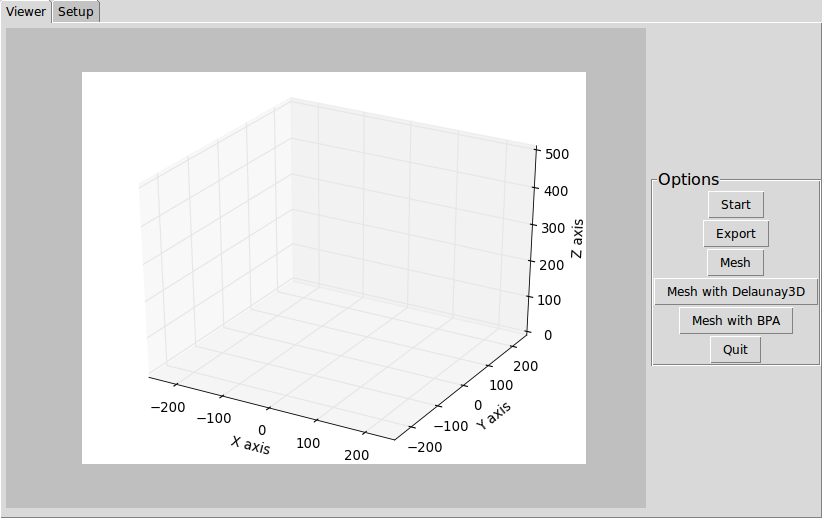
\includegraphics[width=.45\textwidth]{gui-viewer.png}
    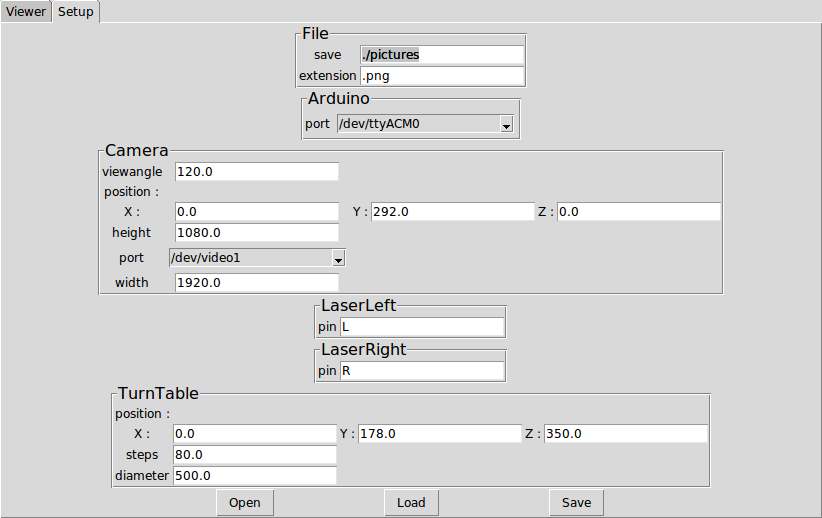
\includegraphics[width=.45\textwidth]{gui-settings.png}
    \caption{\label{fig:gui} L'interface graphique du programme d'acquisition 3D.}
\end{figure}

\chapter{Discussion des résultats}

Dans ce chapitre, nous allons comparer les résultats du scan d'un même objet, en utilisant différents algorithmes et différents paramètres. Pour chacun d'eux, le nombre de points, de faces et le temps de calcul approximatif seront donnés, ainsi qu'un commentaire qualitatif. L'objet choisi est une tasse de format "mug", décorée avec des carrés de couleur et le logo d'une chocolaterie allemande. Une photo de la tasse prise par la webcam du scanner est présentée à la figure \ref{fig:camview}.

Notons que pour des détails d'implémentation, les couleurs ne sont pas conservées en sortie de l'algorithme de balle pivotante \cite{Digne}.

\begin{figure}[h!]
	\centering
	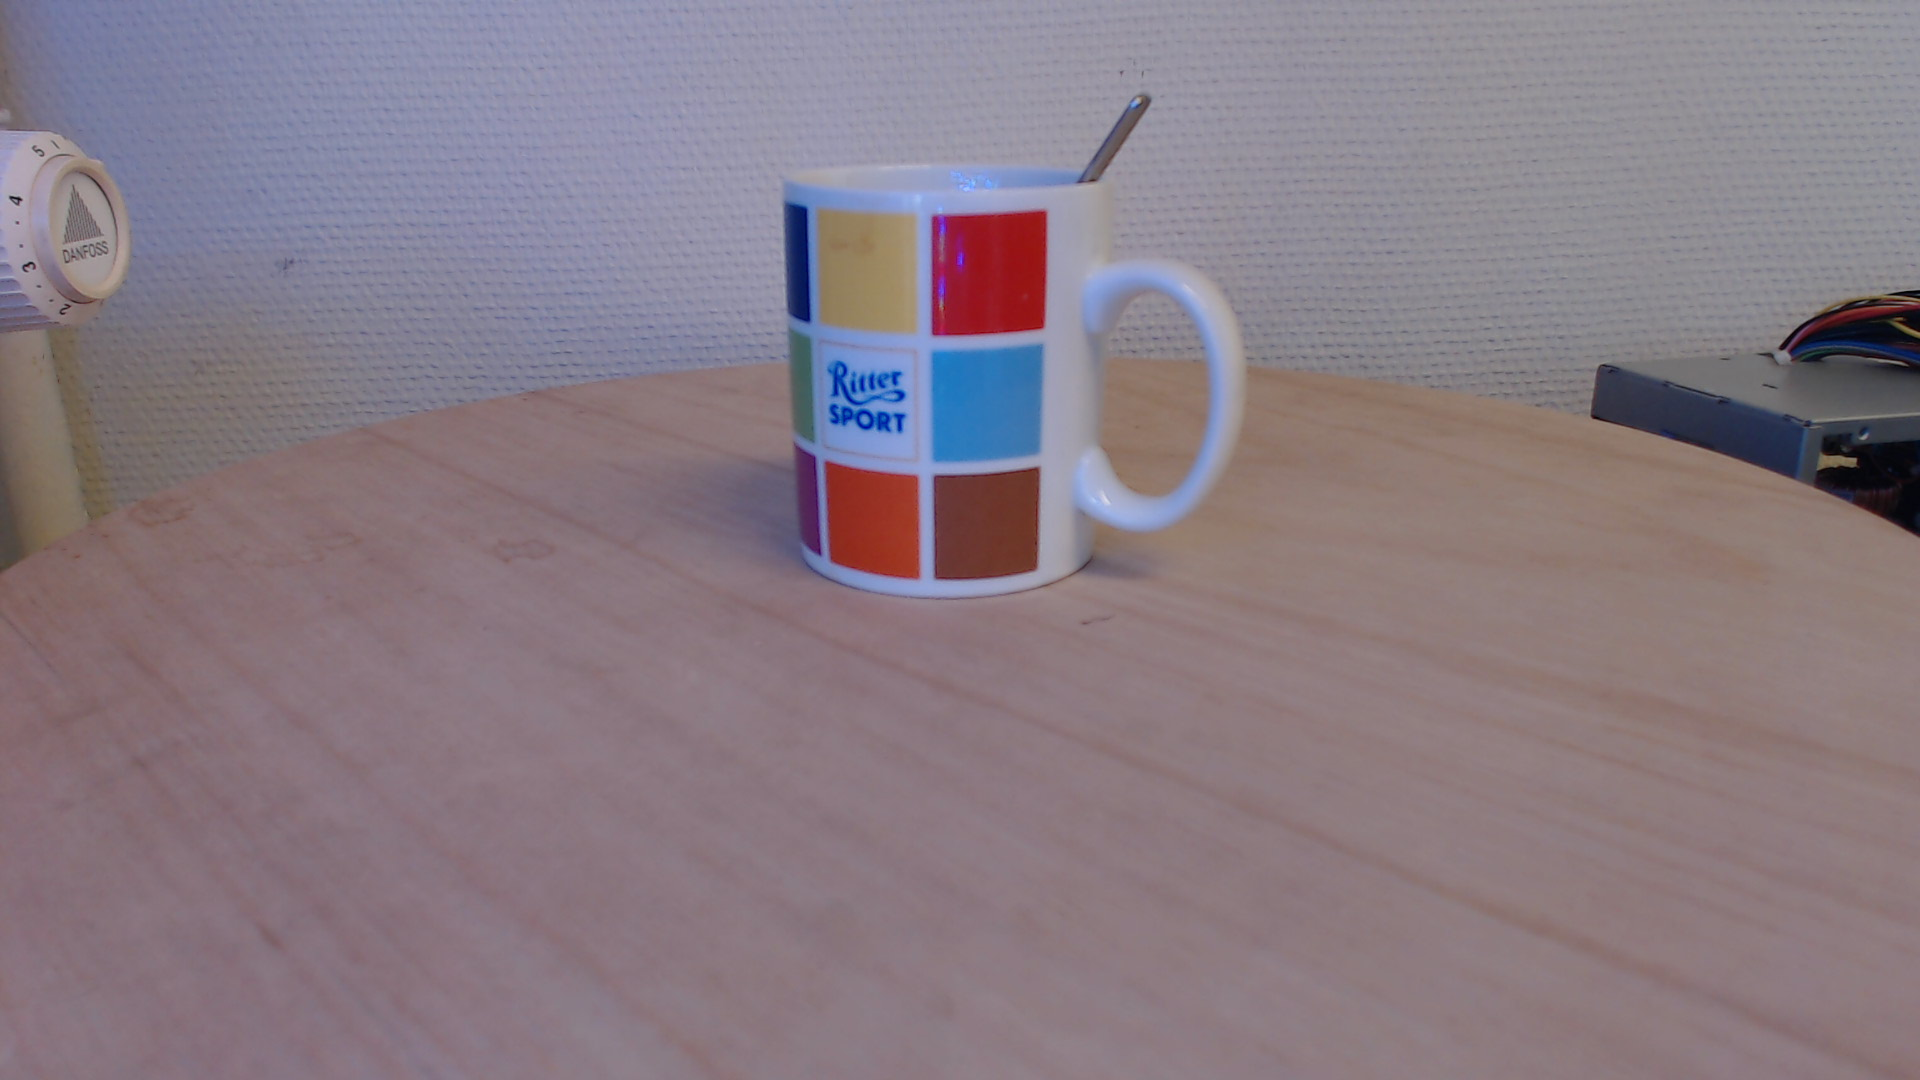
\includegraphics[width=0.7\textwidth]{results/camview.png}
	\caption{\label{fig:camview} Vue de l'objet de test par la webcam du scanner}
\end{figure}

\section{Réglages par défaut du programme}
\subsection{Paramètres}
Sauf mention contraire, les paramètres des comparaison de ce chapitre sont identiques à ceux fixés ci-dessous.

\begin{itemize}
	 \item Seuil pour le filtrage des points par Douglas-Peucker: 2mm
    \item VoxelSpace découpé en cubes de 10mm de côté
    \item z-valeur pour le filtre après l'IPD: 2.58 (99\% d'une distribution normale $\Rightarrow$ longueur maximale de 58mm.
    \item Rayon de balle pour le BPA Meshlab: 24mm
    \item Rayons de balles successifs pour le BPA: 10, 20, 50 et 80mm
    \item Paramètre alpha de Delaunay 3D: 10.0
\end{itemize}

\begin{figure}[h!]
	\centering
    \begin{subfigure}[b]{0.3\textwidth}
	    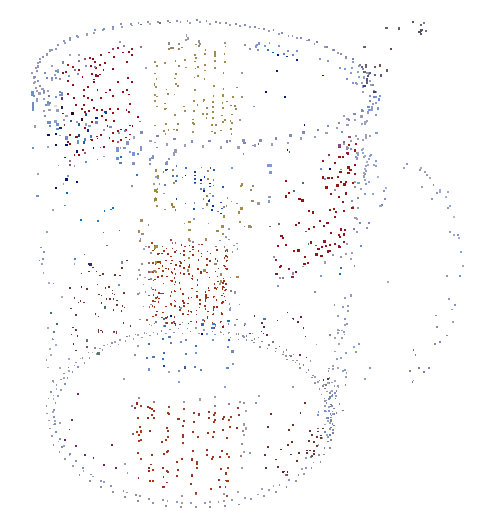
\includegraphics[width=\textwidth]{results/defaults-pointcloud.png}
        \caption{Nuage de points\\1984 points}
    \end{subfigure}
    \begin{subfigure}[b]{0.3\textwidth}
	    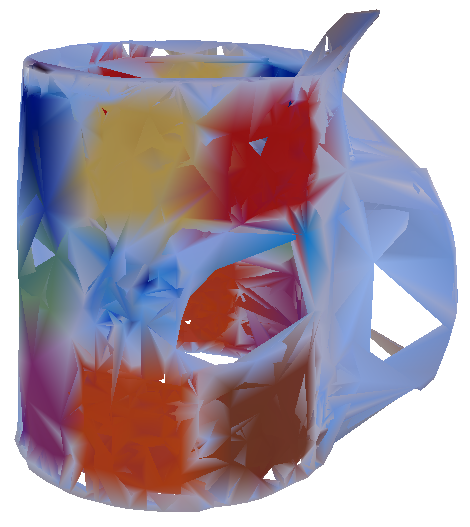
\includegraphics[width=\textwidth]{results/defaults-ipd.png}
        \caption{Intrinsic Property Driven\\11276 faces - 20s}
    \end{subfigure}
    \begin{subfigure}[b]{0.3\textwidth}
	    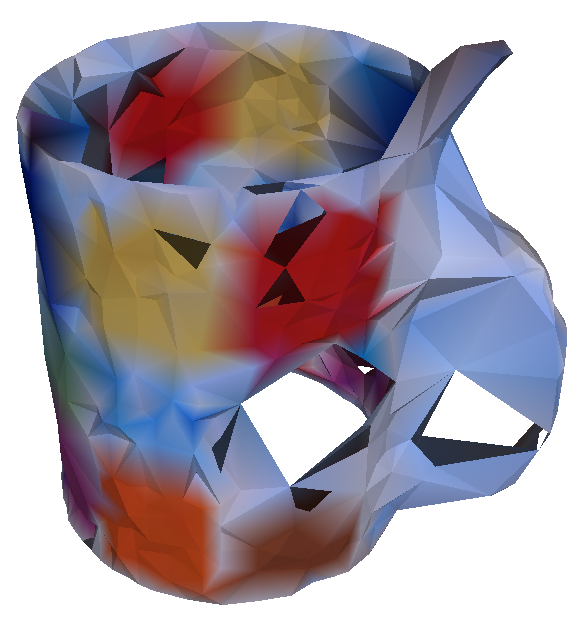
\includegraphics[width=\textwidth]{results/defaults-bpameshlab.png}
        \caption{BPA (Meshlab implementation)\\1961 faces - 1s}
    \end{subfigure}
    \begin{subfigure}[b]{0.3\textwidth}
	    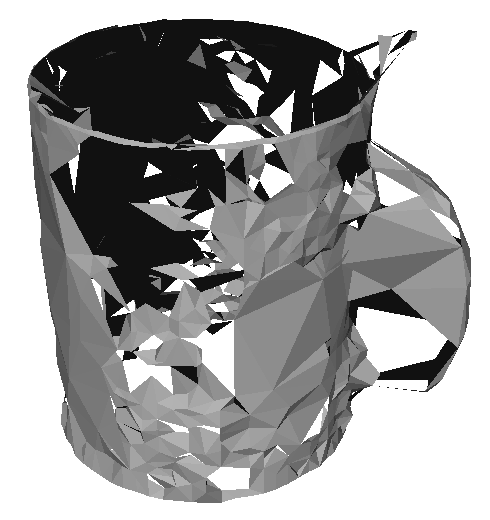
\includegraphics[width=\textwidth]{results/defaults-bpa.png}
        \caption{Ball Pivoting Algorithm\\2102 faces - 1s}
    \end{subfigure}
    \begin{subfigure}[b]{0.3\textwidth}
	    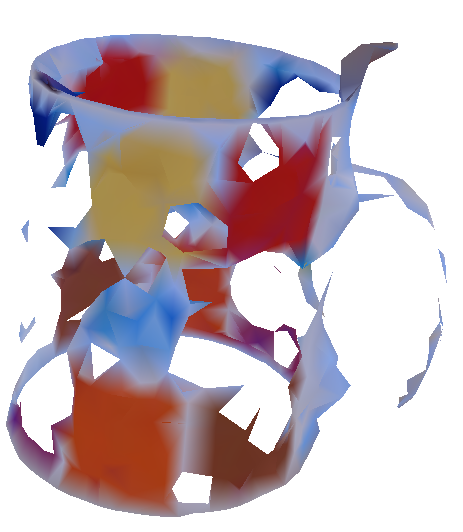
\includegraphics[width=\textwidth]{results/defaults-delaunay.png}
        \caption{Delaunay 3D\\5973 faces - 1s}
    \end{subfigure}
    \caption{\label{fig:meshcmp}Comparaison du maillage avec les différents algorithmes}
\end{figure}

\subsection{Observations}
Les résultats sont présentés à la Figure \ref{fig:meshcmp}
\begin{itemize}
	\item Le nuage de points est peu dense, certaines zones ne sont pas bien couvertes et il semblerait que certaines couleurs soient plus propices a être manquantes que d'autres (tons verts et bleus).
    \item L'algorithme IPD donne de bons résultats, mais il y a beaucoup de triangles, certains se chevauchent. Le temps d'exécution est très supérieur aux autres (voir Figure \ref{fig:meshgraph})
    \item Le BPA donne une surface plus complète que Delaunay 3D, mais avec près de 3 fois moins de faces.
    \item L'implémentation Meshlab laisse de beaucoup moins grands trous que l'implémentation de Julie Digne, bien que cette dernière utilise un rayon de balle progressif.
    \item Delaunay laisse une surface très trouée.
\end{itemize}

\begin{figure}[h!]
	\centering
    \begin{subfigure}[b]{0.4\textwidth}
	    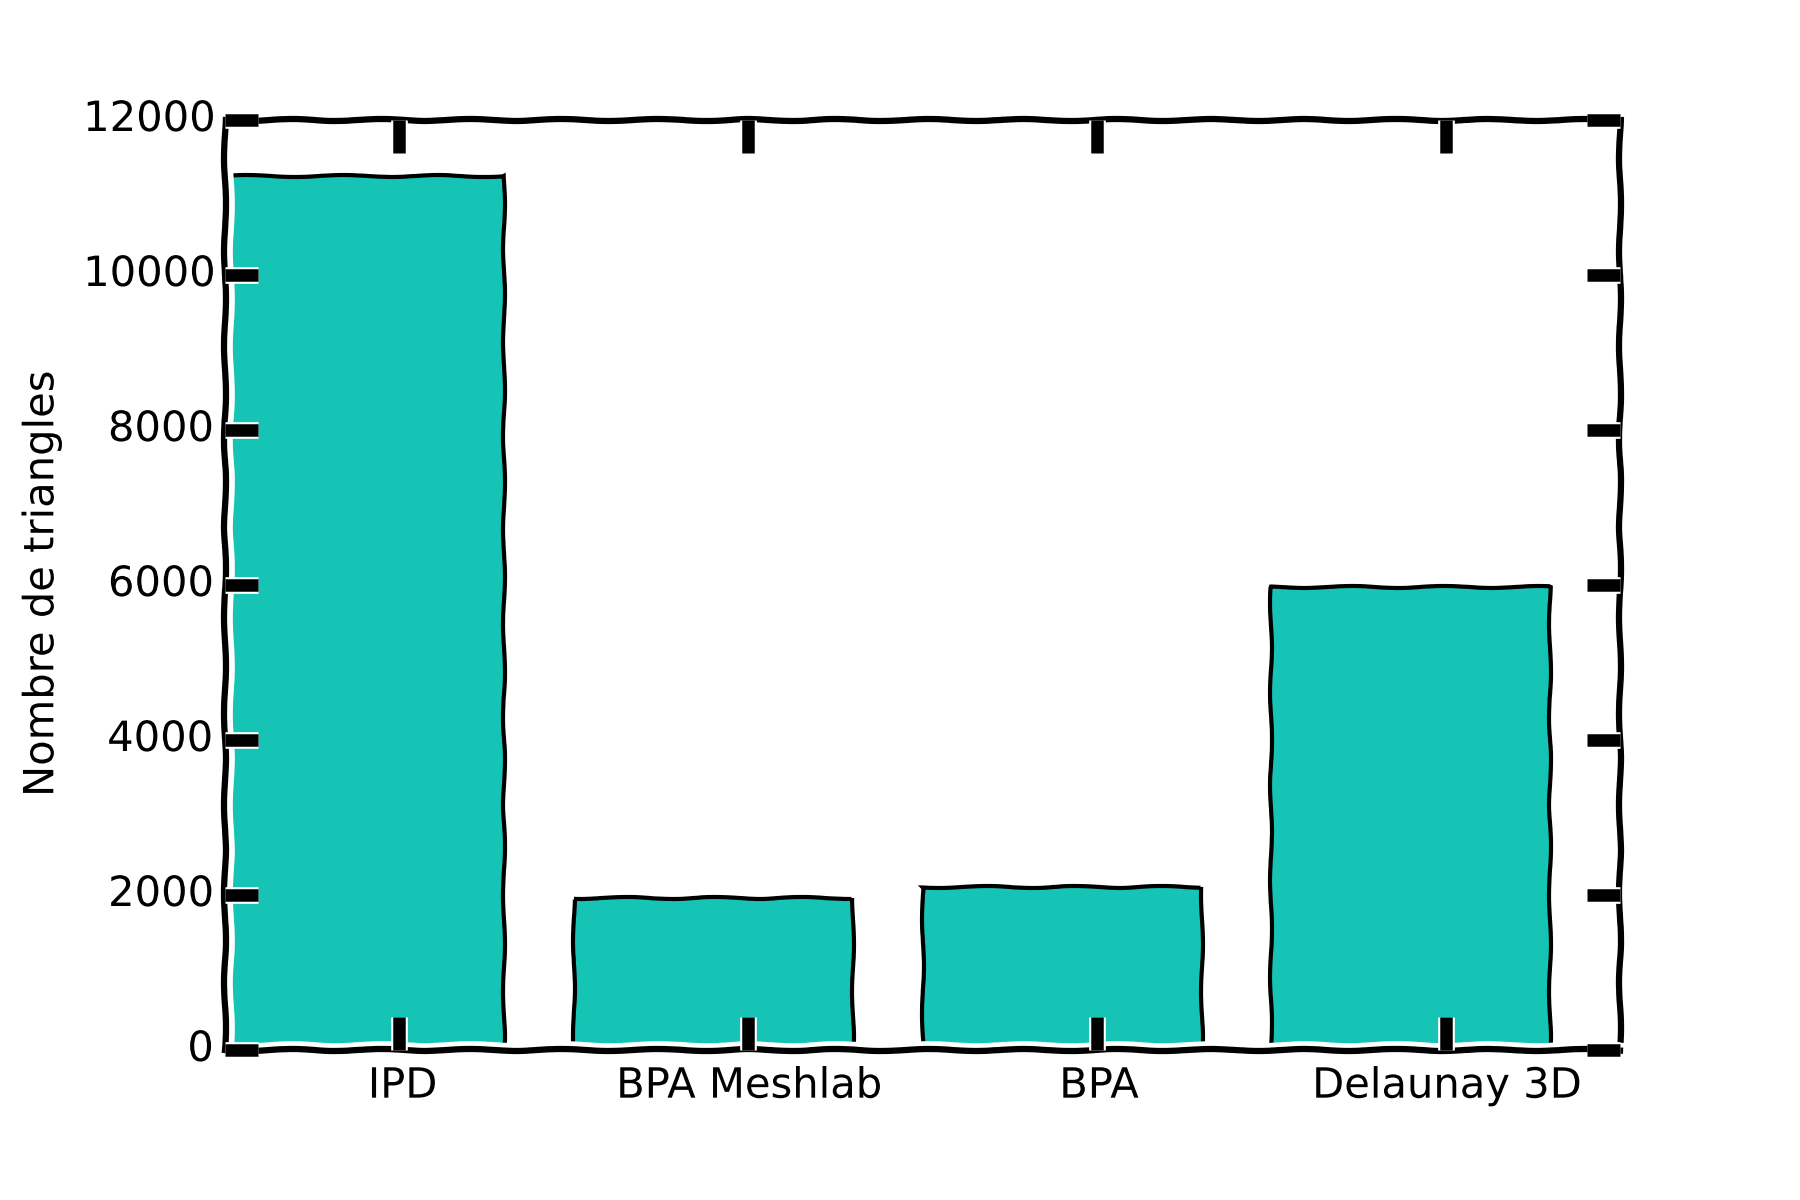
\includegraphics[width=\textwidth]{results/algos-triangles-cmp.png}
        \caption{Nbre de triangles produits}
    \end{subfigure}
    \begin{subfigure}[b]{0.4\textwidth}
	    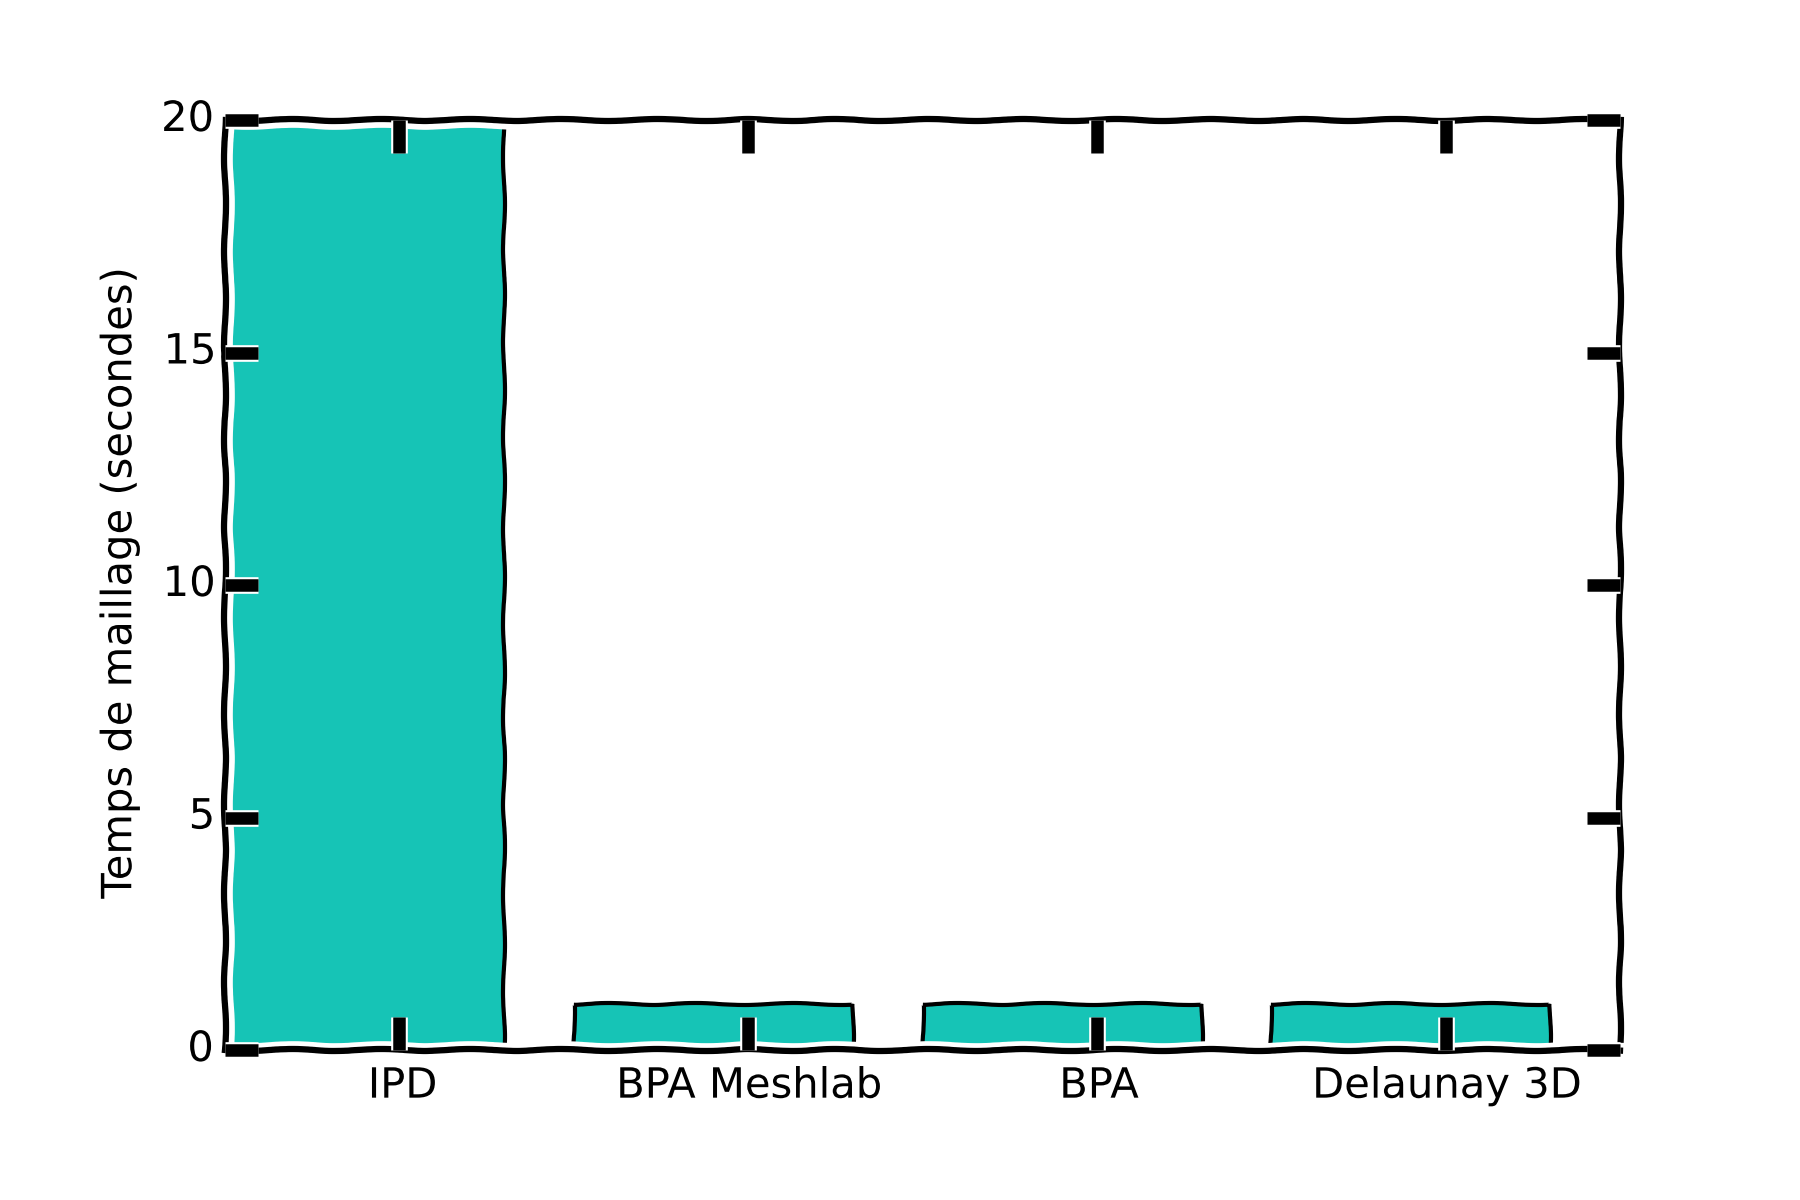
\includegraphics[width=\textwidth]{results/algos-time-cmp.png}
        \caption{Temps d'exécution du maillage}
    \end{subfigure}
    \caption{\label{fig:meshgraph} Comparaison du maillage avec les différents algorithmes - graphes}
\end{figure}

\section{Sans douglas-peucker}
Dans cette variante, on n'utilise pas la simplification de points de Douglas-Peucker (seuil de 0mm). On réduit en outre la taille d'échantillonage du VoxelSpace (structure de données pour la recherche de points dans l'algorithme IPD) à 3mm, pour faire face à l'important nombre de points.

\begin{figure}[h!]
	\centering
    \begin{subfigure}[b]{0.3\textwidth}
	    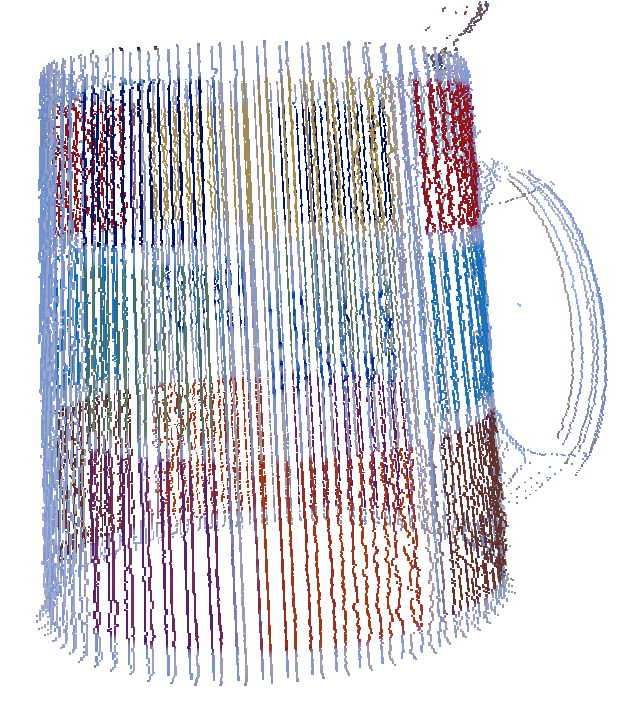
\includegraphics[width=\textwidth]{results/nodp-pointcloud.png}
        \caption{Nuage de points\\62842 points}
    \end{subfigure}
    \begin{subfigure}[b]{0.3\textwidth}
	    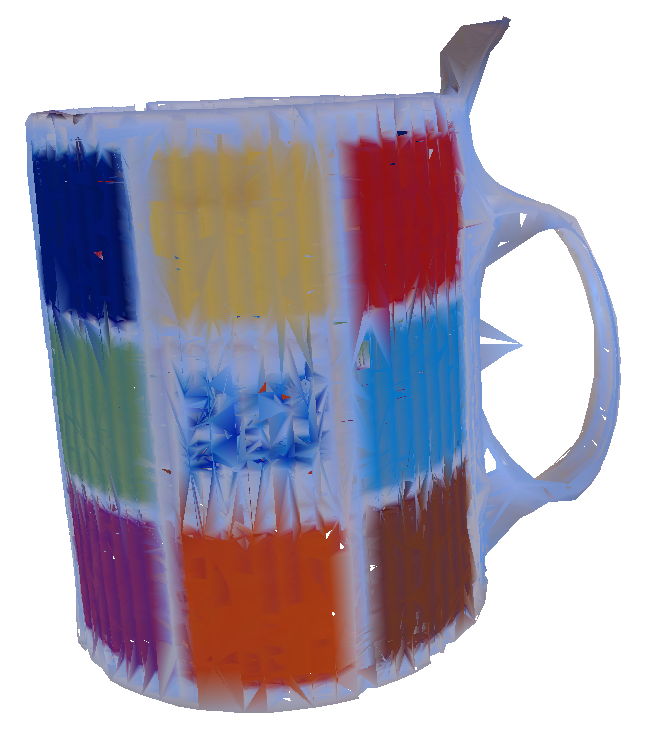
\includegraphics[width=\textwidth]{results/nodp-ipd.png}
        \caption{Intrinsic Property Driven\\487304 faces - 1h48m}
    \end{subfigure}
    \begin{subfigure}[b]{0.3\textwidth}
	    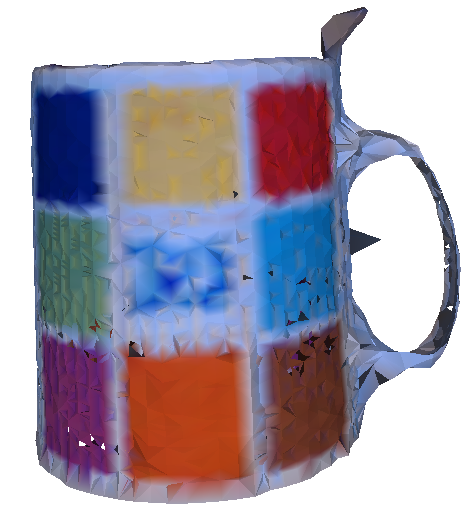
\includegraphics[width=\textwidth]{results/nodp-bpameshlab.png}
        \caption{BPA (Meshlab implementation)\\24168 faces - 15s}
    \end{subfigure}
    \begin{subfigure}[b]{0.3\textwidth}
	    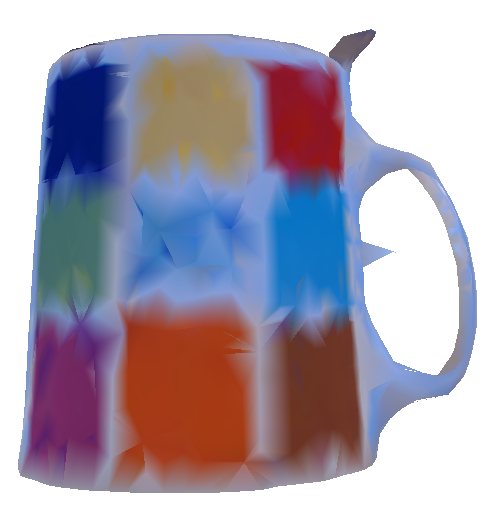
\includegraphics[width=\textwidth]{results/nodp-delaunay.png}
        \caption{Delaunay 3D\\149393 faces - 30s}
    \end{subfigure}
    \begin{subfigure}[b]{0.3\textwidth}
	    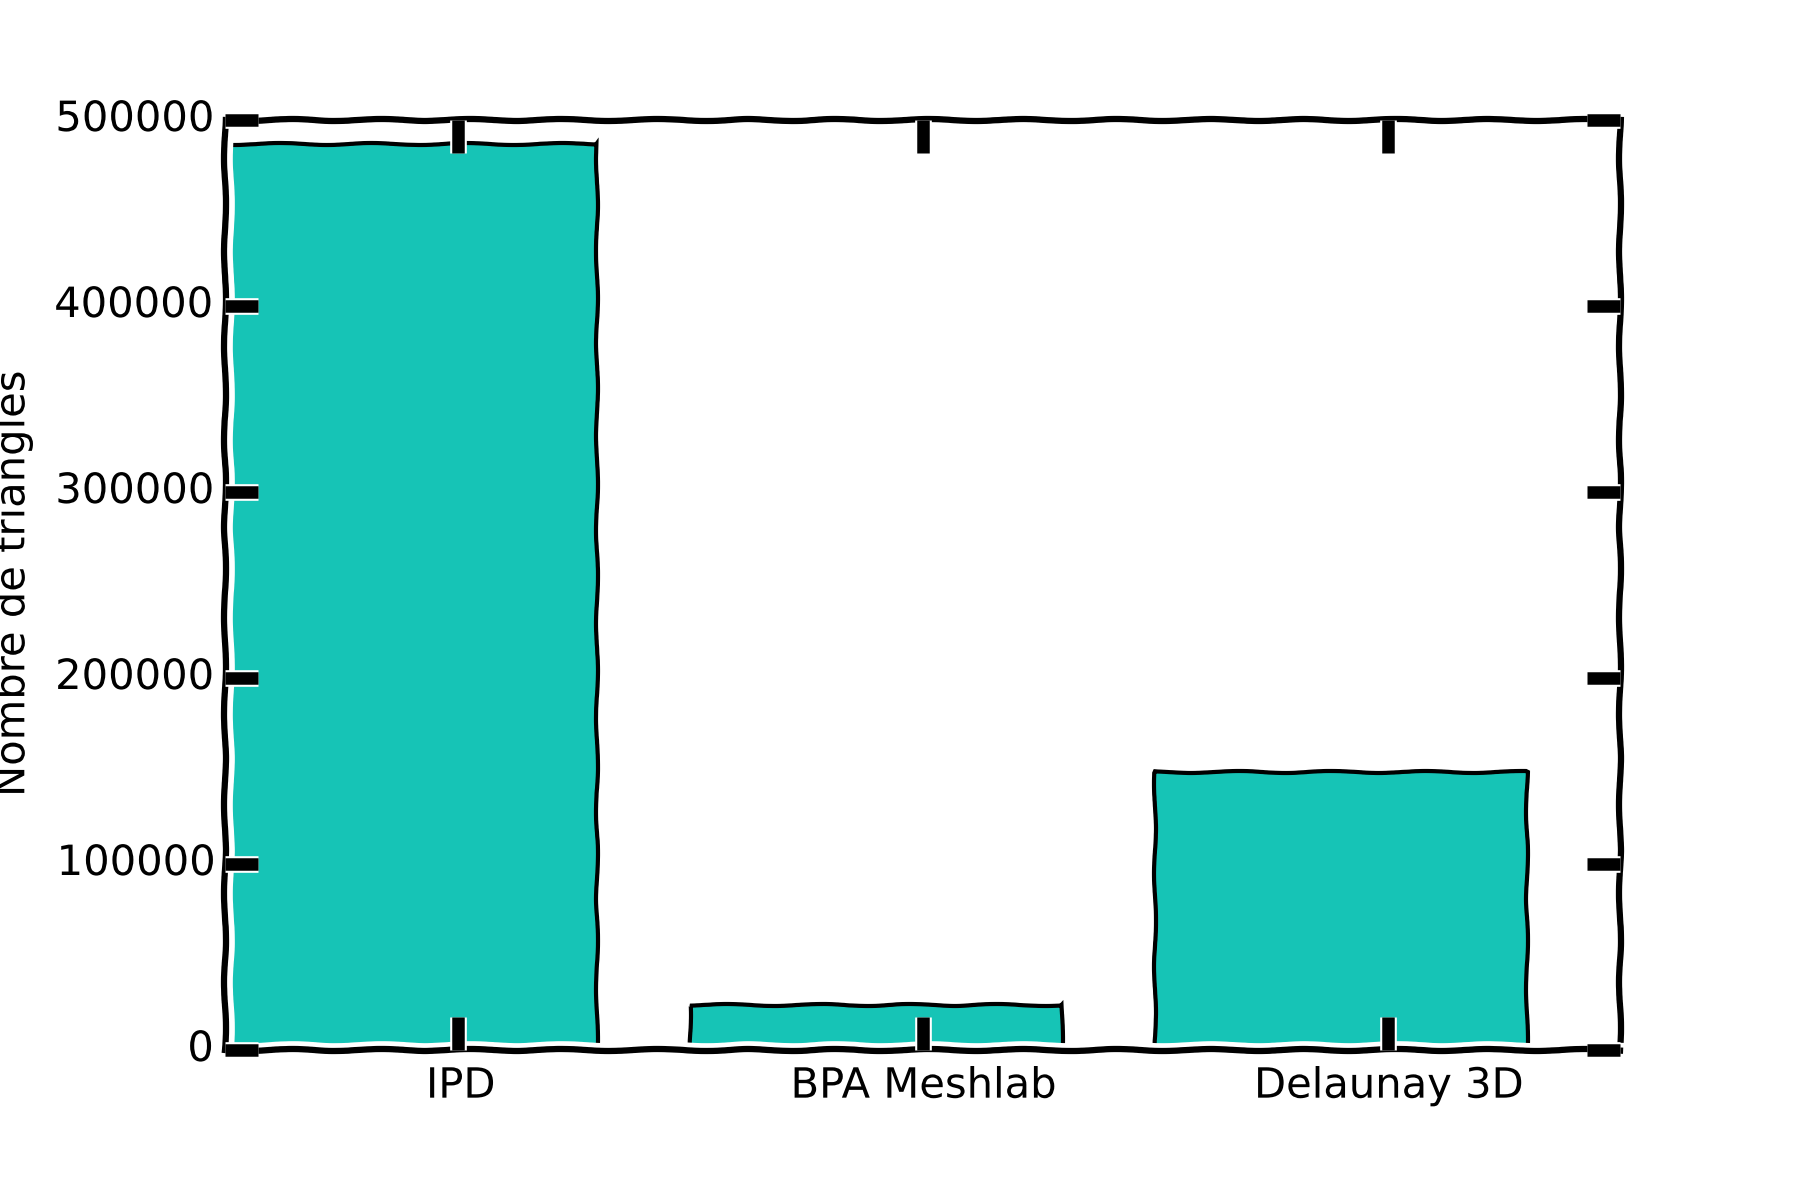
\includegraphics[width=\textwidth]{results/algos-nodp-triangles-cmp.png}
        \caption{Nbre de triangles produits}
    \end{subfigure}
    \begin{subfigure}[b]{0.3\textwidth}
	    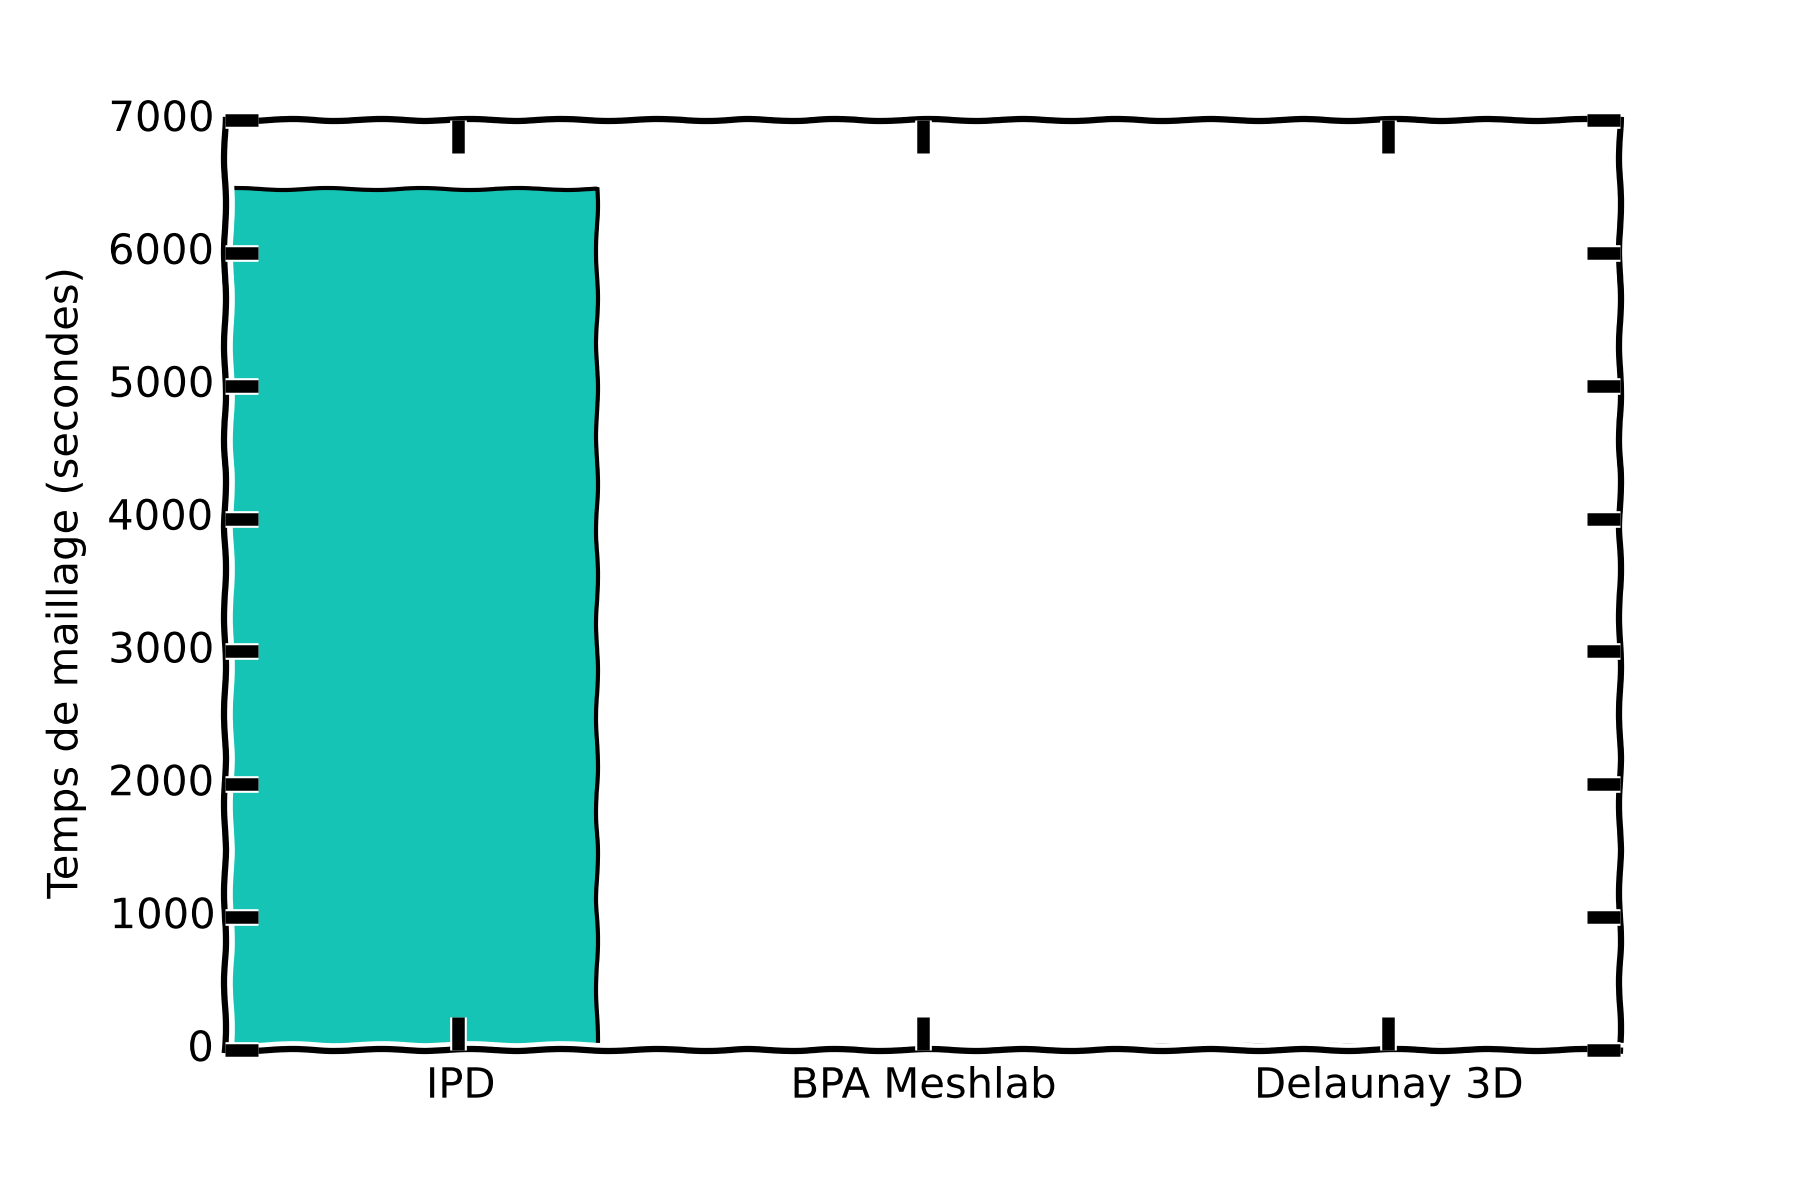
\includegraphics[width=\textwidth]{results/algos-nodp-time-cmp.png}
        \caption{Temps d'exécution du maillage}
    \end{subfigure}
    \caption{\label{fig:meshcmp2}Comparaison du maillage pour les différents algorithmes, sans filtrage préalable des points}
\end{figure}

\subsection{Observations}
Les résultats sont présentés à la Figure \ref{fig:meshcmp2}
\begin{itemize}
	\item Le nuage de point est dense, on peut distinguer les différentes tranches, et toute la surface est bien couverte.
    \item Les régions trouées à la section précédente sont visibles ici, les points y sont bien alignés. C'est donc que l'algorithme de Douglas Peucker a retiré beaucoup de points dans ces zones. Le laser produit donc des résultats différents selon les couleurs qu'il touche.
    \item Le maillage par balle pivotante dans Meshlab donne un résultat beaucoup plus proche de l'objet original. Il n'est cependant pas encore possible de lire le texte.
    \item Notre implémentation en Python du maillage IPD prend beaucoup de temps et génère beaucoup de triangles. Ces triangles sont en outre de mauvaise qualité car on peut voir des sauts de couleur et on distingue les tranches.
    \item L'algorithme BPA intégré à notre programme (\cite{Digne}) ne s'est pas terminé après plusieurs heures, nous n'avons pas obtenu de résultat.
\end{itemize}

\section{Comparaison de différents seuils pour l'algorithme de Douglas Peucker}

Dans cette section, nous comparons le nombre de points obtenus après l'étape de filtrage des point suivant la triangulation, en fonction de la distance minimum à la ligne pour qu'un point soit significatif.

\begin{figure}[h!]
	\centering
    \begin{subfigure}[b]{0.3\textwidth}
	    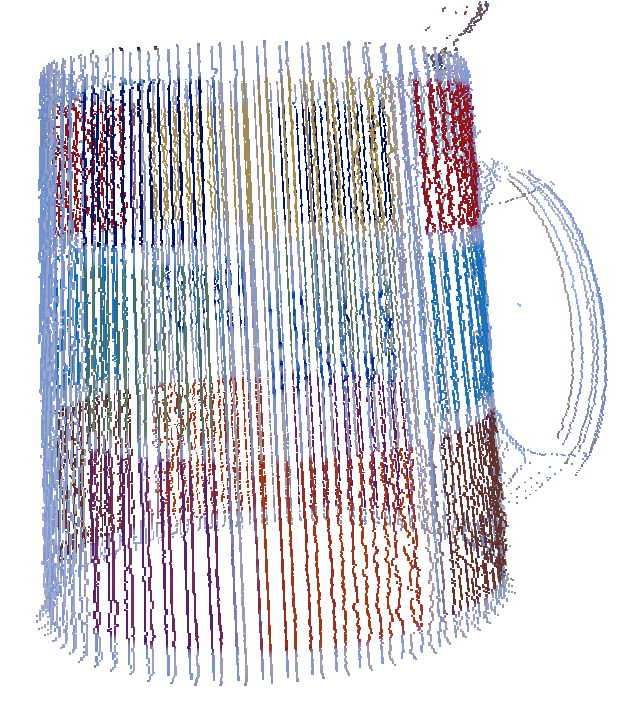
\includegraphics[width=\textwidth]{results/nodp-pointcloud.png}
        \caption{Sans Douglas-Peucker\\62842 points}
    \end{subfigure}
    \begin{subfigure}[b]{0.3\textwidth}
	    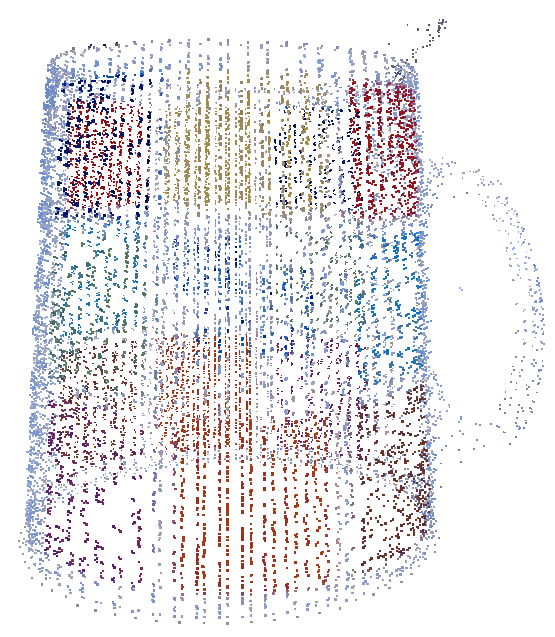
\includegraphics[width=\textwidth]{results/dp05-pointcloud.png}
        \caption{Seuil = 0.5mm\\15215 points}
    \end{subfigure}
    \begin{subfigure}[b]{0.3\textwidth}
	    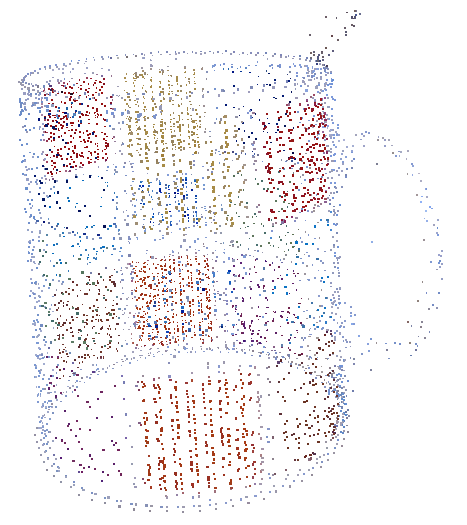
\includegraphics[width=\textwidth]{results/dp1-pointcloud.png}
        \caption{Seuil = 1mm\\5076 points}
    \end{subfigure}
    \begin{subfigure}[b]{0.3\textwidth}
	    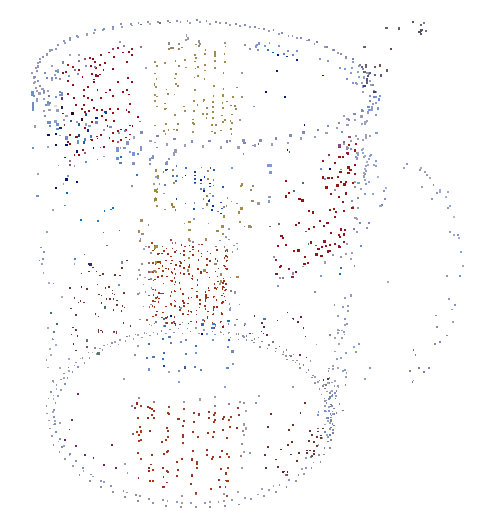
\includegraphics[width=\textwidth]{results/defaults-pointcloud.png}
        \caption{Seuil = 2mm\\1984 points}
    \end{subfigure}
    \begin{subfigure}[b]{0.3\textwidth}
	    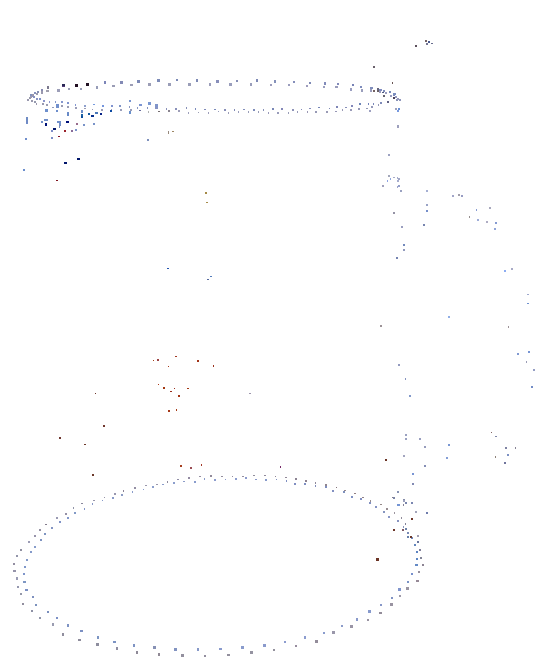
\includegraphics[width=\textwidth]{results/dp5-pointcloud.png}
        \caption{Seuil = 5mm\\505 points}
    \end{subfigure}
    \begin{subfigure}[b]{0.3\textwidth}
	    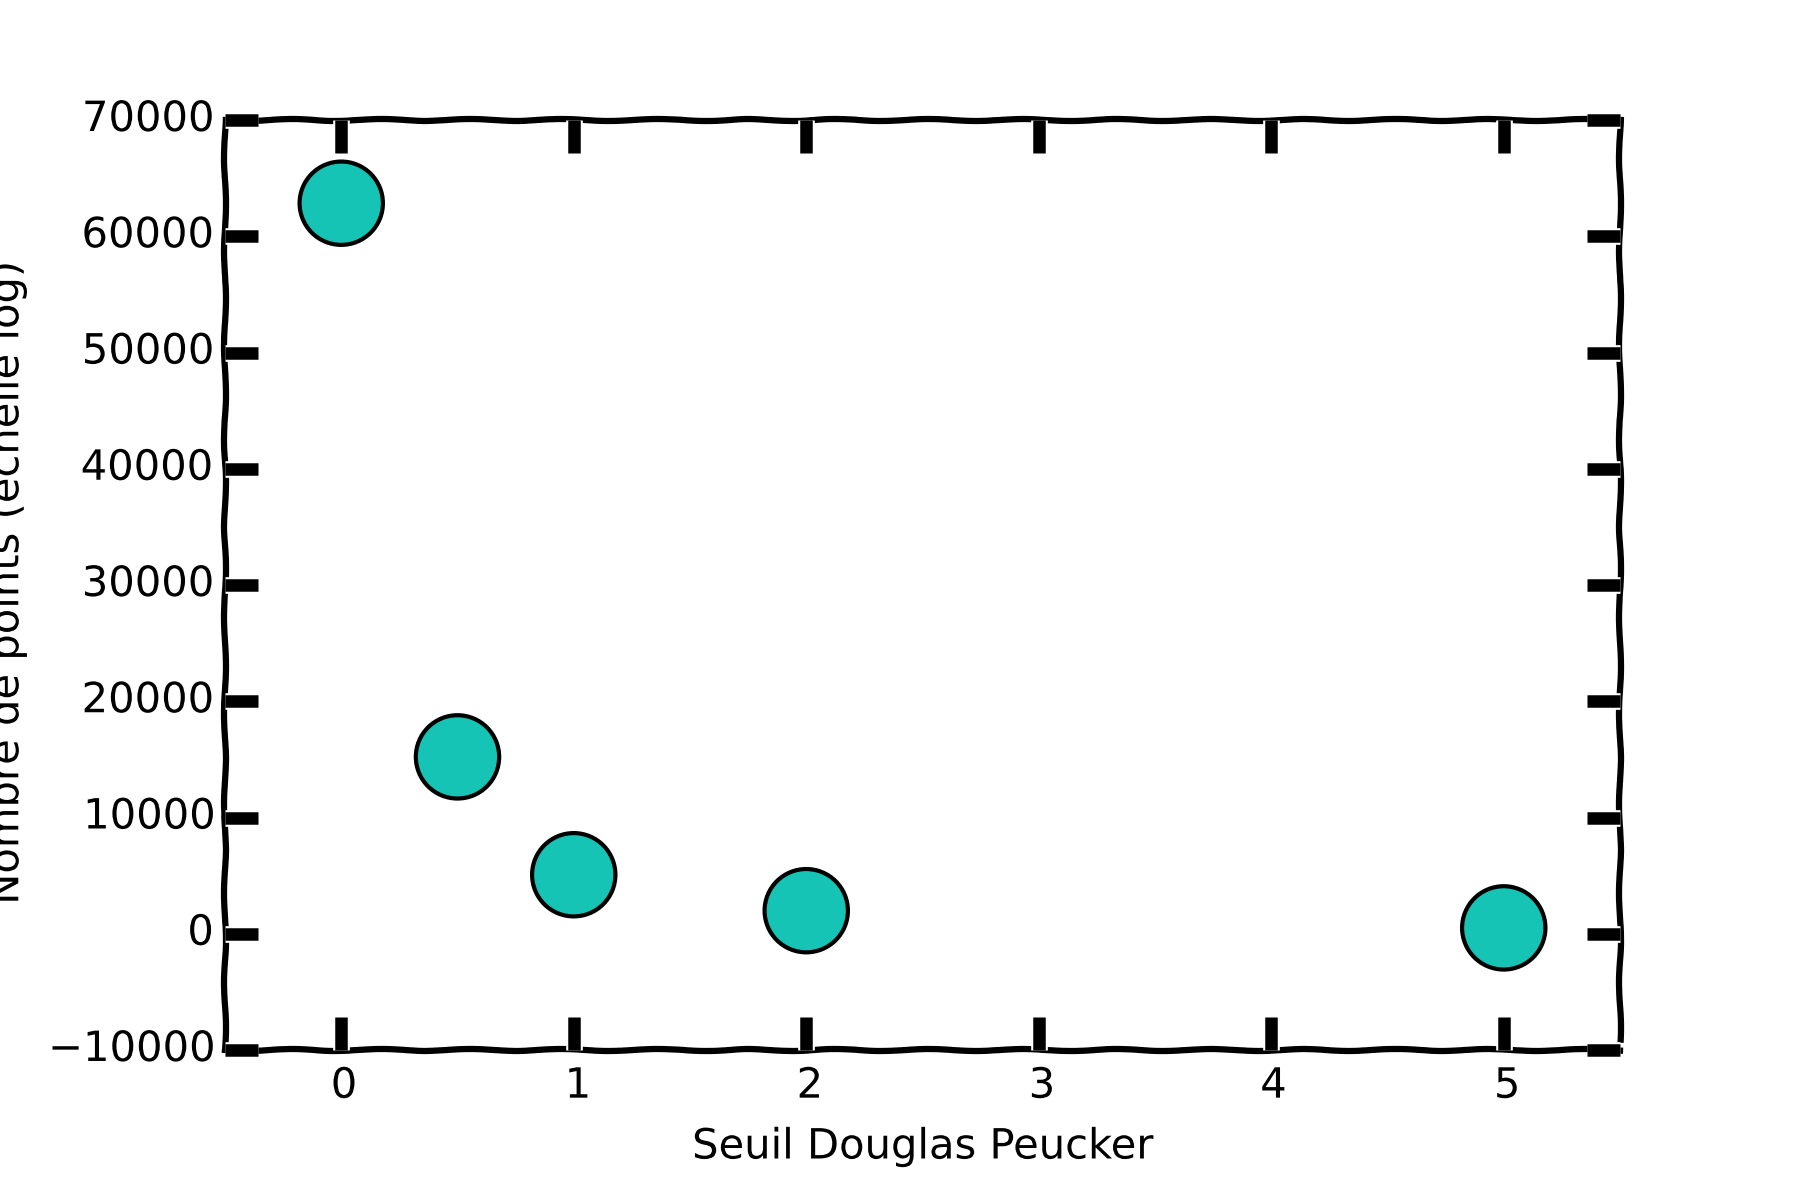
\includegraphics[width=\textwidth]{results/dp-points-graph.png}
        \caption{Nombre de points en fonction du seuil Douglas-Peucker}
    \end{subfigure}
    \caption{\label{fig:dpcmp}Comparaison de différents seuil pour l'étape de filtrage des points par Douglas-Peucker}
\end{figure}

\subsection{Observations}
Les résultats sont présentés à la Figure \ref{fig:dpcmp}
\begin{itemize}
  \item L'algorithme atteint le but fixé, puisque même en retirant beacuoup de points, les significatifs sont gardés
  \item En revanche, la distribution des points supprimés est inégale, probablement car la perception des couleurs par la caméra affecte la précision de la triangulation.
\end{itemize}

\section{Comparaison de différentes tailles de VoxelSpace pour IPD}
Dans cette section, on s'intéresse au temps et au nombre de faces trouvées par notre implémentation Python de l'Intrinsic Property Driver algorithm, lorsqu'on fait varier la taille d'échantillonage du VoxelSpace.

\begin{figure}[h!]
	\centering
    \begin{subfigure}[b]{0.3\textwidth}
	    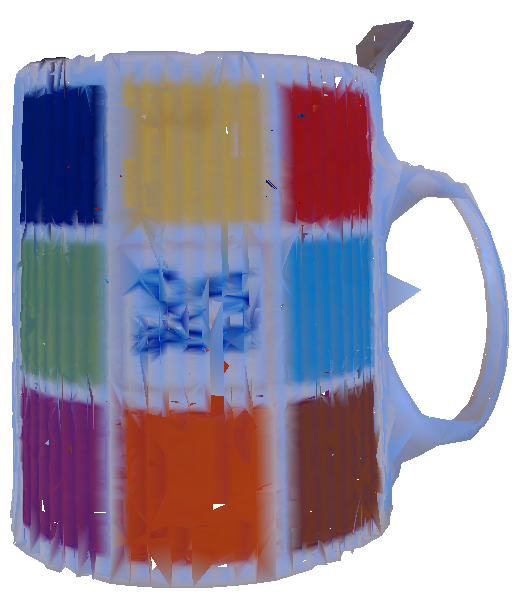
\includegraphics[width=\textwidth]{results/vs05-ipd.png}
        \caption{Cubes de 0.5mm\\356393 faces - 18m59s}
    \end{subfigure}
    \begin{subfigure}[b]{0.3\textwidth}
	    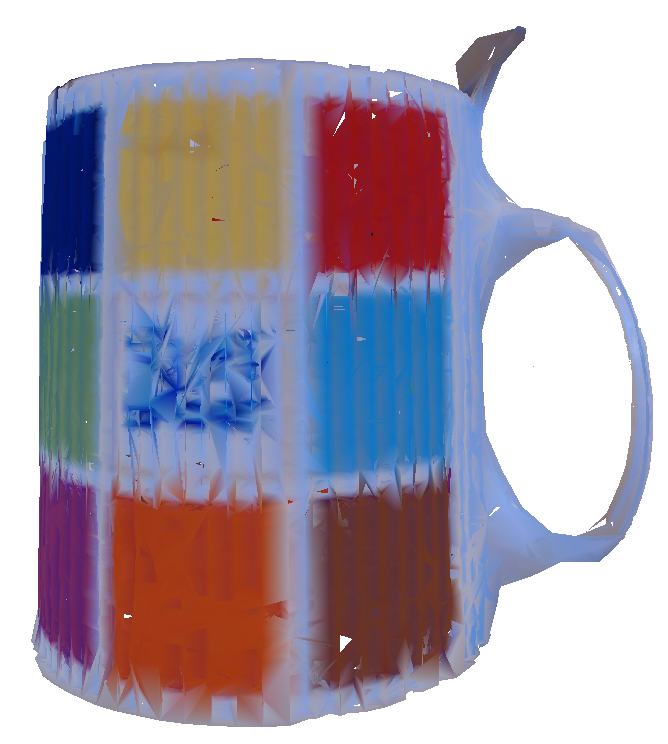
\includegraphics[width=\textwidth]{results/vs1-ipd.png}
        \caption{Cubes de 1mm\\427546 faces - 31m50s}
    \end{subfigure}
    \begin{subfigure}[b]{0.3\textwidth}
	    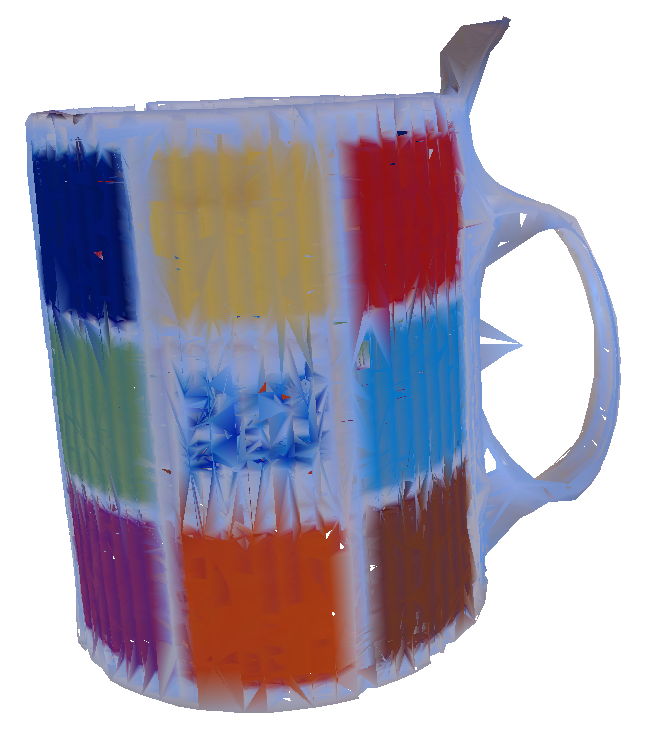
\includegraphics[width=\textwidth]{results/nodp-ipd.png}
        \caption{Cubes de 3mm\\487304 faces - 1h48m}
    \end{subfigure}
    \begin{subfigure}[b]{0.3\textwidth}
	    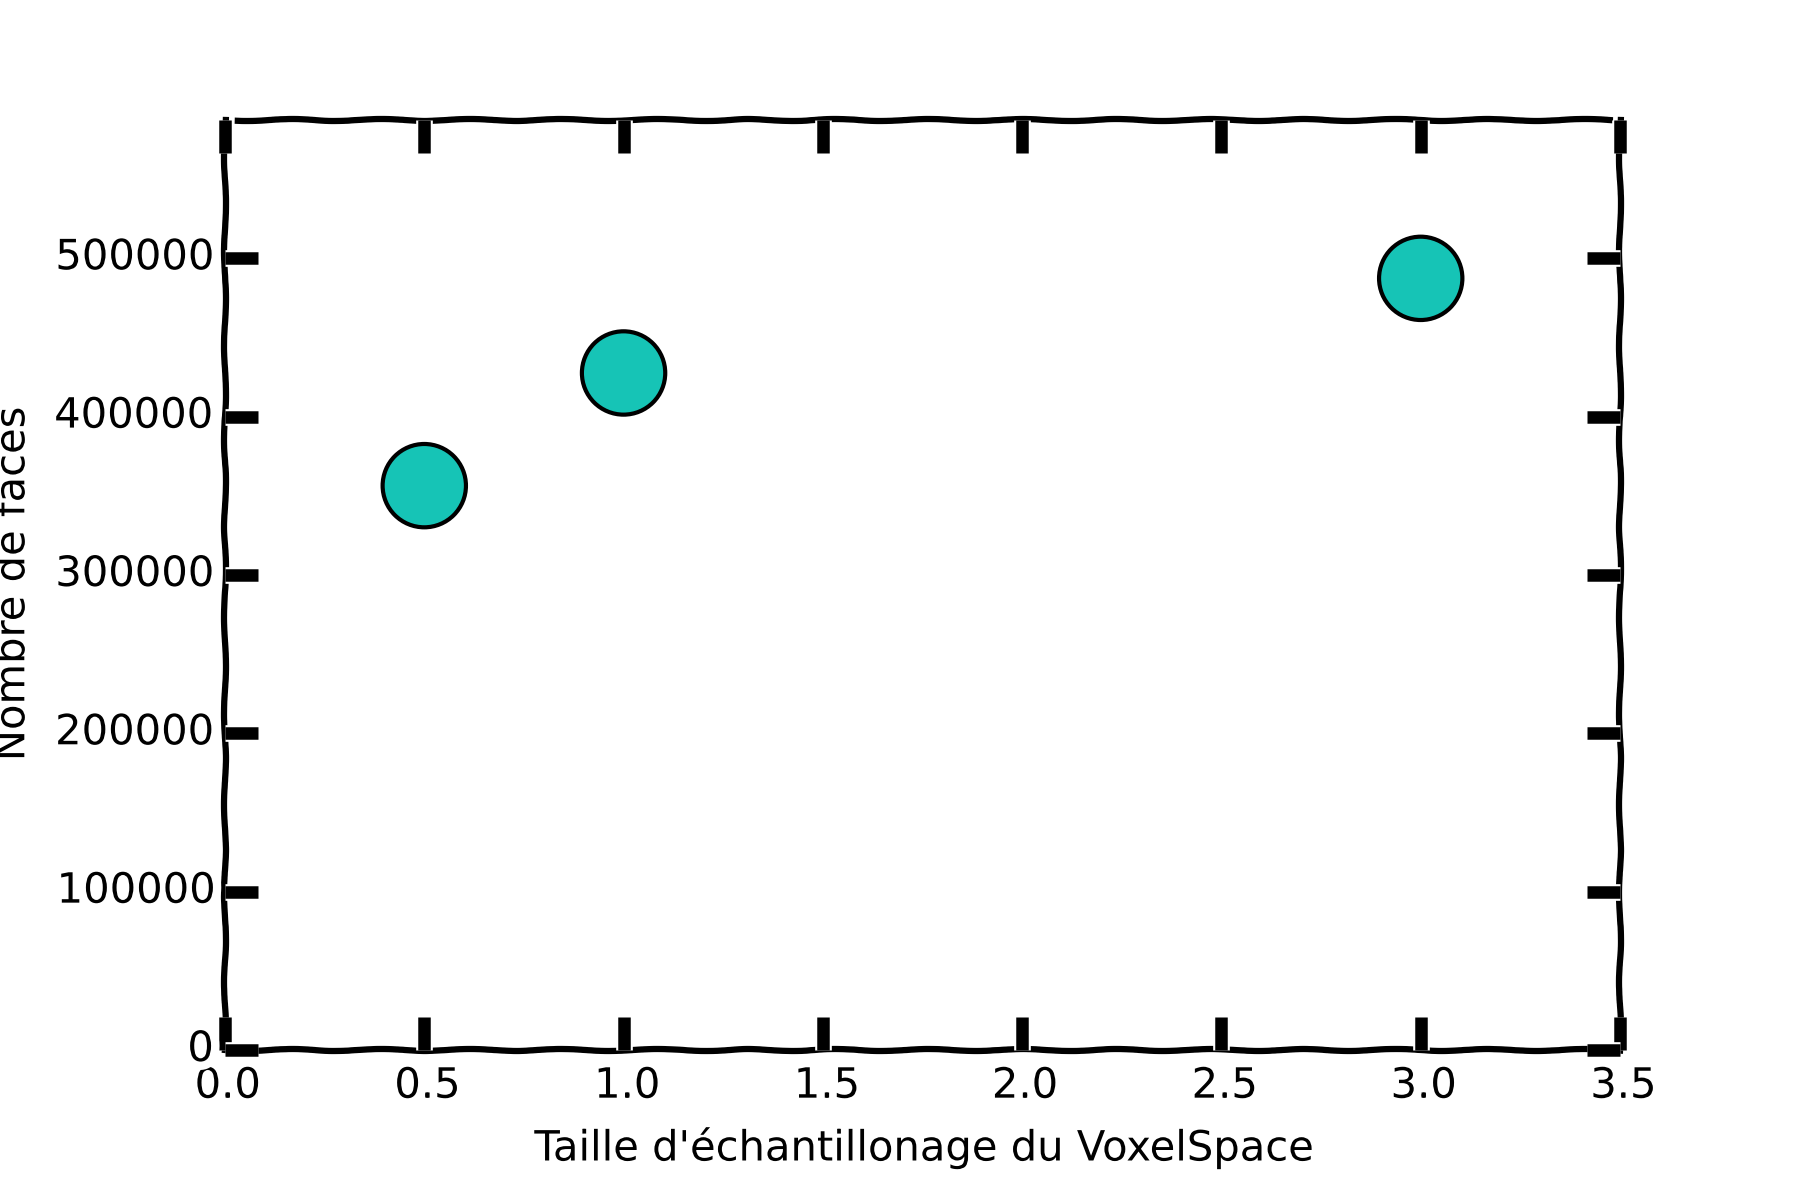
\includegraphics[width=\textwidth]{results/vs-triangles-cmp.png}
        \caption{Nombre de triangles en fonction de la taille du VS}
    \end{subfigure}
    \begin{subfigure}[b]{0.3\textwidth}
	    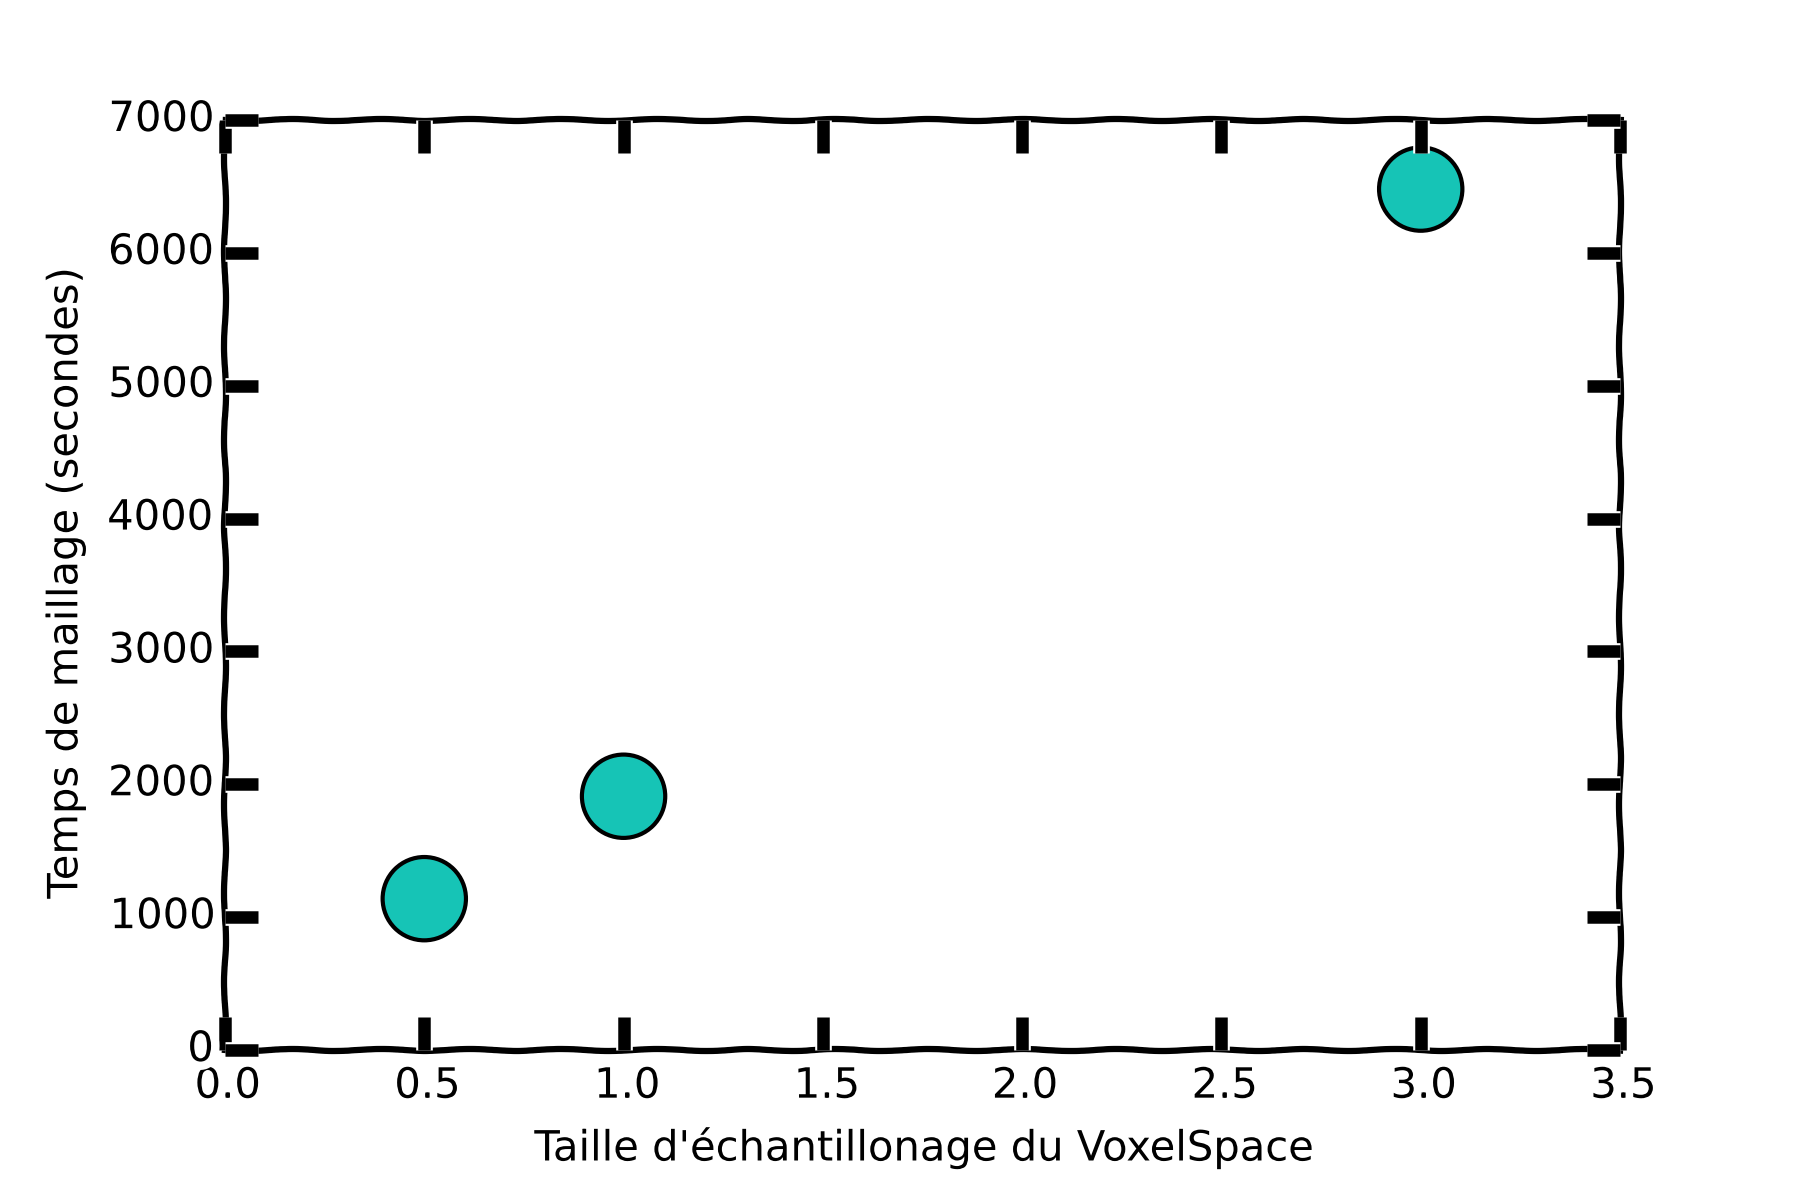
\includegraphics[width=\textwidth]{results/vs-time-cmp.png}
        \caption{Temps de maillage en fonction de la taille du VS}
    \end{subfigure}
    \caption{\label{fig:vscmp} Comparaison des performances et résultats de l'IPD avec différentes tailles de \textit{VoxelSpace}}
\end{figure}

\subsection{Observations}
Les résultats sont présentés à la Figure \ref{fig:vscmp}. De manière générale, la résolution semble trop faible pour obtenir une forme acceptable.

\chapter{Conclusions et perspectives}

Pour une première approche et un premier prototype élaboré à moindre frais, les résultats sont fort satisfaisants. En effet, nous sommes capables de scanner un grand nombre d'objets à surface mate.\\
Bien entendu, les résultats ne sont pas encore "professionnels"; un grand nombre d'améliorations pourraient être encore apportées, notamment:
\begin{itemize}
\item Au niveau hardware, un prototype de meilleure qualité pourrait nettement diminuer le temps d'exécution du scan. En effet, par sa taille et donc son poids, le plateau oscille légèrement lors de la rotation avant de se stabiliser, ce qui nous a forcé à rajouter à chaque pas des délais d'attente de stabilisation avant de pouvoir photographier la scène. En outre, ce temps d'attente ne garantit pas que la structure a arrêté de vibrer, et peut créer un léger flou de mouvement sur les images.
\item La webcam n'est pas entièrement adaptée à la prise de photos précises: l'ajustement automatique de la distance focale et de la balance des blancs peut influencer la qualité des filtres d'extraction des lasers et donc tout le reste de la chaîne.
\item Au niveau de l'extraction des tracés lasers, l'ensemble des filtres pourrait être géré de manière dynamique en fonction du milieu dans lequel le scanner se trouve : il faudrait réaliser une première phase de "calibration d'environnement" afin de déterminer l'intensité lumineuse du milieu pour ensuite estimer au mieux les différents paramètres de filtrage. Malheureusement, ce genre d'opération devrait idéalement se produire pour chaque lot d'images, ce qui risquerait de fortement augmenter le temps du traitement des images. Mais nous pensons que ce genre de traitement pourrait nettement augmenter la qualité des résultats, car il s'agit là d'un problème auquel nous avons souvent été confrontés.
\item Au niveau de la triangulation, nous pourrions effectuer une étude approfondie de la stabilité, du conditionnement et de l'erreur introduite, et les calculs pourraient être remaniés pour réduire au maximum les erreurs.
\item Un post-traitement des points pourrait également être effectué afin de ne conserver que les meilleurs points dès le début et ainsi limiter le temps total de traitement.
\item Au niveau du meshing, on constate que la méthode implémentée est encore relativement lente. Nous pourrions
\end{itemize}

Pour conclure, les résultats de ce premier prototype sont positifs et encouragent à implémenter de nouvelles améliorations afin de rendre les résultats exploitables pour d'autres applications. Nous souhaiterions rendre les objets scannés imprimables par une imprimante 3D, 

\newpage
\appendix

\chapter{Mise en \oe uvre des diodes laser}\label{diodes-laser}
La caractéristique tension/courant en a été mesurée (figure \ref{laser_caracteristique}) sur deux types différents.
Avec un courant ($I_F$) de 15 mA, la quantité de lumière émise paraît suffisante pour notre usage, sans percevoir une surchauffe de la diode (nous ne disposons pas des spécifications du fabriquant quant aux maxima autorisés).\\
Ce courant correspond, pour les diodes vendues dans une enveloppe en laiton sans marque, à une tension de 2,45 V aux bornes de la diode et peut être fourni sans circuit intermédiaire par une sortie de l'arduino (40 mA maximum :  \cite[p.~313]{ATmega}), en interposant en série (figure \ref{laser_circuit}) une résistance($R_F$). Comme elle est en série avec la diode, la différence de potentiel à ses bornes est la tension d'alimentation ($V_A$) dont on déduit la tension de la sortie de l'arduino à l'état bas (V\textsubscript{OL} : \cite[p.~313]{ATmega}) et la tension aux bornes de la diode ($V_F$) :
\begin{equation}
R_F = \frac{V_A-V\textsubscript{OL}-V_F}{I_F} = \frac{5-0,9-2,45}{0,015} \enspace \Omega = 110 \enspace \Omega
\end{equation}

\begin{figure}[h!]
\centering
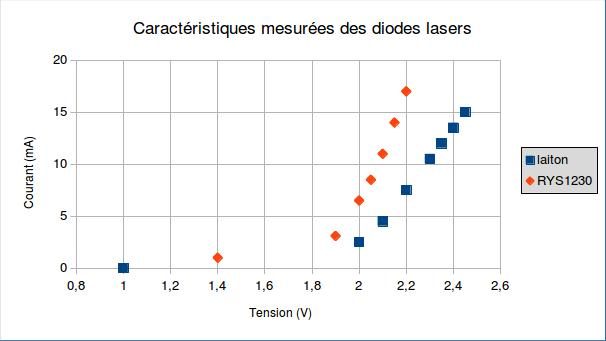
\includegraphics[width=0.8\textwidth]{Caracteristique.jpg}
\caption{Caractéristique mesurée des diodes lasers}
\label{laser_caracteristique}
\end{figure}
\begin{figure}[h!]
\centering
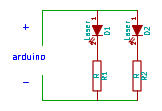
\includegraphics[width=0.4\textwidth]{circuit2lasers.jpg}
\caption{Schéma d'alimentation des diodes laser}
\label{laser_circuit}
\end{figure}
\newpage
\chapter{Le logiciel pour l'arduino}\label{code-arduino}
\begin{lstlisting}
/*
  3DScan
  This driver controls a easydriver
  Commands are :
  r/R: light right laser
  l/L: light left laser
  t/T: turn
  0: shut off both lasers
  b/B: light both lasers
  p/P: put power on
  m/M: put power off
 */

/* Pinout */
static const int dirPin = 2;
static const int stepPin = 3;
static const int laserLeftPin = 12;
static const int laserRightPin = 11;
static const int powerPin = 4;

/* Delay, in milliseconds, to ensure laser state totally changed (on/off time) */
static const int lightDelay = 1;

/* Delay, in microseconds, between each motor half step */
static const int stepDelayMax = 2000;
static const int stepDelayMin = 1500;
static int stepDelay;

/* Delay, in milliseconds to wait after motor turn (plate stabilization) */
static const int afterTurnDelay = 150;

/* Number of steps for a complete rotation */
static const int totalSteps = 8000;

/* Change lasers state */
void laser(int laser_pin, bool value){
  digitalWrite(laser_pin, value ? HIGH : LOW);
  delay(lightDelay);
}

void power(bool on){
  digitalWrite(powerPin, on ? HIGH : LOW);
}

/* Turn platform */
void turn(int n_steps=100){
  int half = n_steps/2;
  int increment = (stepDelayMax - stepDelayMin) / half;
  stepDelay = stepDelayMax;

  for (; n_steps>0; n_steps--){
    digitalWrite(stepPin, HIGH);
    delayMicroseconds(stepDelay);
    digitalWrite(stepPin, LOW);
    delayMicroseconds(stepDelay);
    if (n_steps > half)
      stepDelay -= increment;
    else
      stepDelay += increment;
  }
  delay(afterTurnDelay);
}

void setup() {
  Serial.begin(115200);
  pinMode(dirPin, OUTPUT);
  digitalWrite(dirPin, HIGH);
  pinMode(stepPin, OUTPUT);
  digitalWrite(stepPin, LOW);
  pinMode(laserLeftPin, OUTPUT);
  pinMode(laserRightPin, OUTPUT);
  pinMode(powerPin, OUTPUT);
  digitalWrite(powerPin, LOW);
  laser(false, false);
}

char cmd = 0;
bool ok = true;
void loop() {
  if (Serial.available() > 0){
    ok = true;
    cmd = Serial.read();
    switch (cmd) {
      case '0':
        laser(laserLeftPin, false);
        laser(laserRightPin, false);
        break;

      case 'b':
      case 'B':
        laser(laserLeftPin, true);
        laser(laserRightPin, true);
        break;

      case 'l':
        laser(laserLeftPin, false);
        break;
      case 'L':
        laser(laserLeftPin, true);
        break;

      case 'r':
        laser(laserRightPin, false);
        break;
      case 'R':
        laser(laserRightPin, true);
        break;

      case 't':
      case 'T':
        turn();
        break;

      case 'p':
      case 'P':
        power(true);
        break;

      case 'm':
      case 'M':
        power(false);
        break;

      /* Unknow command*/
      default: 
        ok = false;
    }
    /* Echo back if command suceeded */
    if (ok) 
      Serial.println(cmd);
  }      
}
\end{lstlisting}

\listoffigures

\newpage
\bibliographystyle{apalike}
\bibliography{mybiblio}
\addcontentsline{toc}{chapter}{Bibliographie}
\begin{thebibliography}{1}
\bibitem{shapiro} Shapiro Linda et Stockman G. 2000 "Computer Vision" Prentice Hall
\bibitem{salvi} Salvi Joaquim, Armangué X et Batlle J. 2002 "A comparative review of camera calibrating methods with accuracy evaluation" Elsevier Pattern Recognition 35
\bibitem{tsai} Tsai Roger 1987 "A versatile Camera Calibration Technique for High-accuracy 3D Machine Vision Metrology using off-the-shelf TV Cameras and Lenses" IEEE Journal of Robotics and Automation vol RA-3 n.4 Aug. 87
\bibitem{forest2002} Forest Josep et Salvi J. "A review of laser scanning three-dimensional digitisers" Proceedings of the IEEE/RSJ intl. Conf. on Intelligent Robots and Systems EPFL2002.
\bibitem{forest2004} Forest Josep 2004 "New methods for triangulation-based shape acquisition using laser scanners" Université de Girona; Espagne.
\bibitem{faugeras} Faugeras 1993 "Three-Dimensional Computer Vision - A Geometric Viewpoint" The MIT Press.
\bibitem{sato} Sato Yukio, Kitagawa H. et Fujita H. 1982 "Shape measurement of curved objects using multiple slit-ray projections" IEEE Transactions on Pattern Analysis and Machine Intelligence PAMI-4(6) pp. 641-646.
\bibitem{dsls} Park Johnny, DeSouza G.N. et Kak A.C. 2001 "Dual-beam structured-light scanning for 3-D object modeling" Proceedings Third International Conference on 3-D Digital Imaging and Modeling 2001.
\bibitem{puget} Puget P. et Skordas T. 1990 "Calibrating a mobile camera" ACM Journal Image and Vision Computing Volume 8 Issue 4, November, 1990 pp. 341-348.
\bibitem{jain} Jain Ramesh, Kasturi R et Schunck B. 1995 "Machine Vision" Mcgraw-Hill.
\bibitem{Forsyth} Forsyth David et Ponce J. 2012 "Computer Vision - A Modern Approach" 2e édit. Pearson.
\bibitem{Wei} Wei Zhenehong, Zhou F. et Zhang G. 2005 "3D coordinates measurement based on structured light sensor" Elsevier Sensors and Actuators A 120 (2005) pp. 527-535.
\bibitem{wohler} Wöhler Christian 2009 "3D Computer Vision - Efficient Methods and Applications" Springer.
\bibitem{Murale} Van Gool Luc, Pollefeys M., Proesmans M. et Zalesny A. "The MURALE Project: Image-based 3D modeling for archaeology" 2002 Proceedings of the VAST2000 Euroconference held in Arezzo, November 2000. Oxford, Archaeopress, 2002.
\bibitem{craig} Craig J. 1989 "Introduction to Robotics, Mechanics and Control" Addison-Wesley.
\bibitem{buset} Buset Dominique "Algèbre linéaire" PUB Ecole polytechnique
\bibitem{hartley} Hartley Richard et Zisserman A. 2003 "Multiple View Geometry in Computer Vision" 2e éd. Cambridge University Press.
\bibitem{sturm} Sturm Peter et Maybank S. 1999 "On plane-based camera Calibration: a general Algorithm, Singularities, Applications" IEEE Conference on Computer Vision and Pattern Recognition (CVPR '99), June 1999
\bibitem{Robotic} Nüchter Andreas 2009 "3D Robotic Mapping The Simultaneous Localization and Mapping Problem with Six Degrees of Freedom" Springer Tracs in advanced robotics vol. 52 2009.
\bibitem{Malhotra} Malhotra Akash, Gupta K. et Kant K. 2011 "Laser Triangulation for 3D Profiling of Target" IJCA vol 35-8, pp. 47-50, Dec. 2011.
\bibitem{Voxelization} Haumont D. et Warzée N. "Complete polygonal Scene Voxelization" Journal of Graphics Tools, 7(3), 2002
\bibitem{pulli} Pulli Kari et Shapiro L. 2000 "Surface Reconstruction and Display from Range and Color Data" Academic Press Graphical Models 62
\bibitem{basdogan} Basdogan Cagatay 2007 "From 2D Images to 3D tangible Models: Autostereoscopic and haptic Visualization of Martian Rocks in virtual Environments" MIT Press Presence vol. 16 Febr. 2007
\bibitem{wikiscan3d} \url{http://fr.wikipedia.org/wiki/Scanner_tridimensionnel}
\bibitem{stereo} \url{http://photo.stereo.free.fr/stereoscopie/stereoscopie-pratique.php}
\bibitem{raspberry} \url{http://www.raspberrypi.org/real-time-depth-perception-with-the-compute-module/}
\bibitem{clemson} \url{http://www.clemson.edu/restoration/wlcc/equipment_services/equipment/3d_scanning_and_analysis.html}
\bibitem{rubicon} \url{http://www.rubitech.org/}
\bibitem{ATmega} \url{http://www.atmel.com/images/Atmel-8271-8-bit-AVR-Microcontroller-ATmega48A-48PA-88A-88PA-168A-168PA-328-328P_datasheet_Complete.pdf}
\bibitem{openCV} \url{http://opencv.org/}
\bibitem{opengl} \url{https://www.opengl.org/}
\bibitem{stepper} \url{https://learn.adafruit.com/all-about-stepper-motors}
\bibitem{stepctrl} \url{http://www.st.com/web/en/resource/technical/document/application_note/CD00003774.pdf}
\bibitem{jones_stepper} \url{http://homepage.cs.uiowa.edu/~jones/step/}
\bibitem{UVC} \url{https://help.ubuntu.com/community/Webcam}
\bibitem{gPhoto} \url{http://www.gphoto.org/}
\bibitem{libgp2} \url{http://magiclantern.wikia.com/wiki/Remote_control_with_PTP_and_Python}
\bibitem{cremote} \url{https://pythonhosted.org/canon-remote/}
\bibitem{meshlab} \url{http://meshlab.sourceforge.net/}
\bibitem{vtk} The visualization toolkit \url{http://www.vtk.org/}
\bibitem{Delaunay} \url{http://www.ai.univ-paris8.fr/~audibert/ens/11-Triangulation.pdf}
\bibitem{2algo} Lee D.T. et Schachter B.J. 1980 "Two Algorithms for Constructing a Delaunay Triangulation" International Journal of Computer and Information Sciences vol.9 n.3 Plenum Publishing Corporation
\bibitem{edelsbrunner} Edelsbrunner Herbert, Kirkpatrick D.G. et Seidel R. 1983 "On the Shape of a Set of Points in the Plane" IEEE Transactions on Information Theory vol. IT-29 n.4 juillet 1983.
\bibitem{alpha} Fischer Kaspar 2000 "Introduction to Alpha Shapes" \url{http://www.cs.uu.nl/docs/vakken/ddm/texts/Delaunay/alphashapes.pdf}.
\bibitem{glace} Laloux Martin 2015 "Sur la création des enveloppes concaves (concave hull) et les divers moyens d'y parvenir (formes alpha, alpha shapes)" \url{http://www.portailsig.org/content/sur-la-creation-des-enveloppes-concaves-concave-hull-et-les-divers-moyens-d-y-parvenir-forme} 09-01-2015
\bibitem{bpa} Bernardini Fausto, Mittleman J., Rushmeier H., Silva C. et Taubin G. 1999 "The Ball-Pivoting Algorithm for Surface Reconstruction" IEEE Transactions on Visualization and Computer Graphics oct. 1999, pp. 349-359.
\bibitem{Digne} Digne Julie 2014 "An Analysis and Implementation of a parallelBall pivoting Algorithm" Image Processing On Line juillet 2014.
\bibitem{Berger} Berger Matthew, Tagliasacchi A., Seversky L., Alliez P., Levine J., Sharf A. et Silva C. 2014 "State of the Art in Surface Reconstruction from Point Clouds" Eurographics 2014.
\bibitem{Mencl} Mencl Robert et M{\"u}ller 1998 "Interpolation and Approximation of Surfaces from Three-Dimensional scattered Data Points" State of the Art Reports, Eurographics'98 pp.51-67.
\bibitem{IPD} Lin Hong-Wei, Tai C.L. et Wang G.J. 2004 "A Mesh Reconstruction Algorithm driven by an intrinsic Property of a Point Cloud" Computer-Aided Design vol.36 1-9 Elsevier.
\bibitem{DBRG} Kuo Chuan-Chu et Yau H.T. 2005 "A Delaunay-based Region-growing Approach to Surface Reconstruction from unorganized Points" Computer-Aided Design v.37 pp.825-835.
\bibitem{douglaspeucker} David H. Douglas et Thomas K. Peucker 1973 "Algorithm for the reduction of the number of points required to represent a digitized line or its caricature" 1973 Cartographica: The International Journal for Geographic Information and Geovisualization Volume 10, Number 2 / December 1973.

\textbf{Références non exploitées (provenant des recherches initiales) :}
\bibitem{Poisson} Kazhdan Michael, Bolitho M. et Hoppe H. 2006 "Poisson Surface Reconstruction" Proceedings Symposium on Geometry 2006, pp. 61–70.
\bibitem{Zhang} Zhang Guangjun et Wei Z. 2002 "A novel calibration approach to structured light 3D vision inspection" Elsevier Optics and Laser Technology 34 (2002) pp. 373-380.
\bibitem{Fuchs} Fuchs A., Grussenmeyer P., Kadi H. et Perrin J.-P. 2004 "Architectural modelling and archaeological reconstitution: digital tools for 3d acquisition and modelling assistance" Workshop on Vision Techniques Applied to the Rehabilitation of City Centres, Oct. 2004, lisbonne, Portugal. pp.1-12.
\bibitem{Biometrics} Zhang David et Lu G. 2013 "3D Biometrics Systems and Applications" Springer 2013.
\bibitem{Irecos} Debeir Olivier, Dunham P., Engels L., Leloup T., Baele X. et Warzée N. 2007 "High resolution 3D acquisition of the Olivier Strebelle's sculpture Athletes' Alley in Beijing 2008" International Review on Computers and Software Vol. 2, 5, pp. 541-545, Sept 2007.
\bibitem{Bathow} Bathow Christiane et Breuckmann B. "High-Definition 3D Acquisition of archaeological Objects an Overview of various challenging Projects all over the World" 2011 Proceedings XXIII CIPA Symposium - Prague, Czech Republic - Sept. 2011.
\begin{comment}
\subsection{A novel calibration approach to structured light 3D vision inspection}
Une bonne calibration du dispositif est essentielle pour assurer une précision correcte; cet article en décrit une méthode.(\cite{Zhang})
\subsection{3D coordinates measurement based on structured light sensor}
Cet article présente les bases du calcul de la précision des mesures réalisées avec un laser.(\cite{Wei})
\subsection{3D Robotic Mapping The Simultaneous Localization and Mapping Problem with Six Degrees of Freedom}
Ce petit livre résume les bases mathématiques indispensables pour notre projet.[\cite{Robotic})]
\subsection{Complete polygonal Scene Voxelization}
Cet aricle présente un algorithme heuristique pour déterminer, dans l'espace, les points qui appartiennent à un objet complexe.(\cite{Voxelization})
\subsection{Poisson Surface Reconstruction}
Cet article présente une méthode d'égalisation (smoothing) pour la reconstitution de surfaces à partir de points et d'un quadrillage en éléments finis.(\cite{Poisson})
\subsection{High resolution 3D acquisition of the Olivier Strebelle's sculpture Athletes' Alley in Beijing 2008}
Cet article expose les difficultés rencontrées par le scanning d'une structure complexe et les solutions trouvées.(\cite{Irecos})
\subsection{3D Biometrics Systems and Applications}
La biométrie est un domaine d'application important de la technologie que nous étudions; le chapitre 3 de ce livre démontre en particulier l'utilisation d'un dispositif semblable au nôtre pour la reconnaissance auriculaire et en décrit le fonctionnement.(\cite{Biometrics})
\end{comment}
\end{thebibliography}
\end{document}